\documentclass[a4paper]{book}
\usepackage{makeidx}
\usepackage{graphicx}
\usepackage{multicol}
\usepackage{float}
\usepackage{listings}
\usepackage{color}
\usepackage{ifthen}
\usepackage[table]{xcolor}
\usepackage{textcomp}
\usepackage{alltt}
\usepackage{ifpdf}
\ifpdf
\usepackage[pdftex,
            pagebackref=true,
            colorlinks=true,
            linkcolor=blue,
            unicode
           ]{hyperref}
\else
\usepackage[ps2pdf,
            pagebackref=true,
            colorlinks=true,
            linkcolor=blue,
            unicode
           ]{hyperref}
\usepackage{pspicture}
\fi
\usepackage[utf8]{inputenc}
\usepackage{mathptmx}
\usepackage[scaled=.90]{helvet}
\usepackage{courier}
\usepackage{sectsty}
\usepackage[titles]{tocloft}
\usepackage{doxygen}
\lstset{language=C++,inputencoding=utf8,basicstyle=\footnotesize,breaklines=true,breakatwhitespace=true,tabsize=8,numbers=left }
\makeindex
\setcounter{tocdepth}{3}
\renewcommand{\footrulewidth}{0.4pt}
\renewcommand{\familydefault}{\sfdefault}
\begin{document}
\hypersetup{pageanchor=false}
\begin{titlepage}
\vspace*{7cm}
\begin{center}
{\Large Reference Manual}\\
\vspace*{1cm}
{\large Generated by Doxygen 1.7.4}\\
\vspace*{0.5cm}
{\small Tue May 29 2012 23:03:10}\\
\end{center}
\end{titlepage}
\clearemptydoublepage
\pagenumbering{roman}
\tableofcontents
\clearemptydoublepage
\pagenumbering{arabic}
\hypersetup{pageanchor=true}
\chapter{Class Index}
\section{Class Hierarchy}
This inheritance list is sorted roughly, but not completely, alphabetically:\begin{DoxyCompactList}
\item \contentsline{section}{ColorTranslator}{\pageref{classColorTranslator}}{}
\item \contentsline{section}{Configuration}{\pageref{classConfiguration}}{}
\item \contentsline{section}{ConfigurationHandler}{\pageref{classConfigurationHandler}}{}
\item \contentsline{section}{Display}{\pageref{classDisplay}}{}
\item \contentsline{section}{FileLoader}{\pageref{classFileLoader}}{}
\begin{DoxyCompactList}
\item \contentsline{section}{RawLoader}{\pageref{classRawLoader}}{}
\item \contentsline{section}{X3DLoader}{\pageref{classX3DLoader}}{}
\end{DoxyCompactList}
\item \contentsline{section}{GraphicalObject}{\pageref{classGraphicalObject}}{}
\item \contentsline{section}{KeystoneSetting}{\pageref{structKeystoneSetting}}{}
\item \contentsline{section}{Mat4}{\pageref{structMat4}}{}
\item \contentsline{section}{Monitor}{\pageref{classMonitor}}{}
\item \contentsline{section}{Projector}{\pageref{classProjector}}{}
\item \contentsline{section}{Scene}{\pageref{classScene}}{}
\item \contentsline{section}{Shader}{\pageref{classShader}}{}
\item \contentsline{section}{ThreeDSpace}{\pageref{classThreeDSpace}}{}
\item \contentsline{section}{Uniforms\_\-struct}{\pageref{structUniforms__struct}}{}
\item \contentsline{section}{UniversalConfiguration}{\pageref{classUniversalConfiguration}}{}
\item \contentsline{section}{Vec3}{\pageref{structVec3}}{}
\item \contentsline{section}{Vec3Int}{\pageref{structVec3Int}}{}
\item \contentsline{section}{Vec4}{\pageref{structVec4}}{}
\end{DoxyCompactList}

\chapter{Class Index}
\section{Class List}
Here are the classes, structs, unions and interfaces with brief descriptions:\begin{DoxyCompactList}
\item\contentsline{section}{\hyperlink{classColorTranslator}{ColorTranslator} }{\pageref{classColorTranslator}}{}
\item\contentsline{section}{\hyperlink{classConfiguration}{Configuration} }{\pageref{classConfiguration}}{}
\item\contentsline{section}{\hyperlink{classConfigurationHandler}{ConfigurationHandler} }{\pageref{classConfigurationHandler}}{}
\item\contentsline{section}{\hyperlink{classDisplay}{Display} }{\pageref{classDisplay}}{}
\item\contentsline{section}{\hyperlink{classFileLoader}{FileLoader} }{\pageref{classFileLoader}}{}
\item\contentsline{section}{\hyperlink{classGraphicalObject}{GraphicalObject} }{\pageref{classGraphicalObject}}{}
\item\contentsline{section}{\hyperlink{structKeystoneSetting}{KeystoneSetting} }{\pageref{structKeystoneSetting}}{}
\item\contentsline{section}{\hyperlink{structMat4}{Mat4} }{\pageref{structMat4}}{}
\item\contentsline{section}{\hyperlink{classMonitor}{Monitor} }{\pageref{classMonitor}}{}
\item\contentsline{section}{\hyperlink{classProjector}{Projector} }{\pageref{classProjector}}{}
\item\contentsline{section}{\hyperlink{classRawLoader}{RawLoader} }{\pageref{classRawLoader}}{}
\item\contentsline{section}{\hyperlink{classScene}{Scene} }{\pageref{classScene}}{}
\item\contentsline{section}{\hyperlink{classShader}{Shader} }{\pageref{classShader}}{}
\item\contentsline{section}{\hyperlink{classThreeDSpace}{ThreeDSpace} }{\pageref{classThreeDSpace}}{}
\item\contentsline{section}{\hyperlink{structUniforms__struct}{Uniforms\_\-struct} }{\pageref{structUniforms__struct}}{}
\item\contentsline{section}{\hyperlink{classUniversalConfiguration}{UniversalConfiguration} }{\pageref{classUniversalConfiguration}}{}
\item\contentsline{section}{\hyperlink{structVec3}{Vec3} }{\pageref{structVec3}}{}
\item\contentsline{section}{\hyperlink{structVec3Int}{Vec3Int} }{\pageref{structVec3Int}}{}
\item\contentsline{section}{\hyperlink{structVec4}{Vec4} }{\pageref{structVec4}}{}
\item\contentsline{section}{\hyperlink{classX3DLoader}{X3DLoader} }{\pageref{classX3DLoader}}{}
\end{DoxyCompactList}

\chapter{Class Documentation}
\hypertarget{classColorTranslator}{
\section{ColorTranslator Class Reference}
\label{classColorTranslator}\index{ColorTranslator@{ColorTranslator}}
}
\subsection*{Public Member Functions}
\begin{DoxyCompactItemize}
\item 
\hyperlink{classColorTranslator_a27ca339a756db56b8ad0cf19b6a9a107}{ColorTranslator} ()  throw ( std::string )
\item 
\hyperlink{classColorTranslator_a88aa857f714fa7f09432a97d9bd89e18}{ColorTranslator} (\hyperlink{structVec3}{Vec3} factor)  throw ( std::string )
\item 
\hyperlink{classColorTranslator_ab89af499b7817dff740652eaf17607fa}{$\sim$ColorTranslator} ()
\item 
void \hyperlink{classColorTranslator_a3d4f90452a337a1752917dfeab1be3f8}{setConversionFactor} (\hyperlink{structVec3}{Vec3} factor)  throw ( std::string )
\item 
\hyperlink{structVec3}{Vec3} \hyperlink{classColorTranslator_a5442cbe5dee3420189c7147c987cb44b}{getConversionFactor} () const 
\item 
\hyperlink{classShader}{Shader} $\ast$ \hyperlink{classColorTranslator_afe0270b9b2920771abf823011aebf0c2}{getShader} () const 
\item 
void \hyperlink{classColorTranslator_a8c2067bfbf7adc6dbe70676fbb2e090f}{setFactorUniform} ()
\end{DoxyCompactItemize}


\subsection{Constructor \& Destructor Documentation}
\hypertarget{classColorTranslator_a27ca339a756db56b8ad0cf19b6a9a107}{
\index{ColorTranslator@{ColorTranslator}!ColorTranslator@{ColorTranslator}}
\index{ColorTranslator@{ColorTranslator}!ColorTranslator@{ColorTranslator}}
\subsubsection[{ColorTranslator}]{\setlength{\rightskip}{0pt plus 5cm}ColorTranslator::ColorTranslator (
\begin{DoxyParamCaption}
{}
\end{DoxyParamCaption}
)  throw ( std::string )}}
\label{classColorTranslator_a27ca339a756db56b8ad0cf19b6a9a107}
Constructs a new \hyperlink{classColorTranslator}{ColorTranslator} with a standard conversion factor. \hypertarget{classColorTranslator_a88aa857f714fa7f09432a97d9bd89e18}{
\index{ColorTranslator@{ColorTranslator}!ColorTranslator@{ColorTranslator}}
\index{ColorTranslator@{ColorTranslator}!ColorTranslator@{ColorTranslator}}
\subsubsection[{ColorTranslator}]{\setlength{\rightskip}{0pt plus 5cm}ColorTranslator::ColorTranslator (
\begin{DoxyParamCaption}
\item[{{\bf Vec3}}]{factor}
\end{DoxyParamCaption}
)  throw ( std::string )}}
\label{classColorTranslator_a88aa857f714fa7f09432a97d9bd89e18}
Constructs a new \hyperlink{classColorTranslator}{ColorTranslator} with the given conversion factor. 
\begin{DoxyParams}{Parameters}
{\em factor} & a vector of 3 floats that determine the amount of red, green that will be converted to red. \\
\hline
\end{DoxyParams}
\hypertarget{classColorTranslator_ab89af499b7817dff740652eaf17607fa}{
\index{ColorTranslator@{ColorTranslator}!$\sim$ColorTranslator@{$\sim$ColorTranslator}}
\index{$\sim$ColorTranslator@{$\sim$ColorTranslator}!ColorTranslator@{ColorTranslator}}
\subsubsection[{$\sim$ColorTranslator}]{\setlength{\rightskip}{0pt plus 5cm}ColorTranslator::$\sim$ColorTranslator (
\begin{DoxyParamCaption}
{}
\end{DoxyParamCaption}
)}}
\label{classColorTranslator_ab89af499b7817dff740652eaf17607fa}
Destructor. 

\subsection{Member Function Documentation}
\hypertarget{classColorTranslator_a5442cbe5dee3420189c7147c987cb44b}{
\index{ColorTranslator@{ColorTranslator}!getConversionFactor@{getConversionFactor}}
\index{getConversionFactor@{getConversionFactor}!ColorTranslator@{ColorTranslator}}
\subsubsection[{getConversionFactor}]{\setlength{\rightskip}{0pt plus 5cm}{\bf Vec3} ColorTranslator::getConversionFactor (
\begin{DoxyParamCaption}
{}
\end{DoxyParamCaption}
) const}}
\label{classColorTranslator_a5442cbe5dee3420189c7147c987cb44b}
Returns a pointer to the factor of this class \begin{DoxyReturn}{Returns}
the factor of this class. 
\end{DoxyReturn}
\hypertarget{classColorTranslator_afe0270b9b2920771abf823011aebf0c2}{
\index{ColorTranslator@{ColorTranslator}!getShader@{getShader}}
\index{getShader@{getShader}!ColorTranslator@{ColorTranslator}}
\subsubsection[{getShader}]{\setlength{\rightskip}{0pt plus 5cm}{\bf Shader} $\ast$ ColorTranslator::getShader (
\begin{DoxyParamCaption}
{}
\end{DoxyParamCaption}
) const}}
\label{classColorTranslator_afe0270b9b2920771abf823011aebf0c2}
Returns the pointer to the shader object specified (in case apply method isn't the right approach) \begin{DoxyReturn}{Returns}
a pointer to the shader object of this class. 
\end{DoxyReturn}
\hypertarget{classColorTranslator_a3d4f90452a337a1752917dfeab1be3f8}{
\index{ColorTranslator@{ColorTranslator}!setConversionFactor@{setConversionFactor}}
\index{setConversionFactor@{setConversionFactor}!ColorTranslator@{ColorTranslator}}
\subsubsection[{setConversionFactor}]{\setlength{\rightskip}{0pt plus 5cm}void ColorTranslator::setConversionFactor (
\begin{DoxyParamCaption}
\item[{{\bf Vec3}}]{factor}
\end{DoxyParamCaption}
)  throw ( std::string )}}
\label{classColorTranslator_a3d4f90452a337a1752917dfeab1be3f8}
Sets the factor of this class. If the sum of the components in factor is bigger than 1 normalize the components. 
\begin{DoxyParams}{Parameters}
{\em factor} & a vector of 3 floats that determine the amount of red, green that will be converted to red. \\
\hline
\end{DoxyParams}
\hypertarget{classColorTranslator_a8c2067bfbf7adc6dbe70676fbb2e090f}{
\index{ColorTranslator@{ColorTranslator}!setFactorUniform@{setFactorUniform}}
\index{setFactorUniform@{setFactorUniform}!ColorTranslator@{ColorTranslator}}
\subsubsection[{setFactorUniform}]{\setlength{\rightskip}{0pt plus 5cm}void ColorTranslator::setFactorUniform (
\begin{DoxyParamCaption}
{}
\end{DoxyParamCaption}
)}}
\label{classColorTranslator_a8c2067bfbf7adc6dbe70676fbb2e090f}
Sets the uniform \char`\"{}factor\char`\"{} so that the fragment shader can access the factor of this class. 

The documentation for this class was generated from the following files:\begin{DoxyCompactItemize}
\item 
ColorTranslator.h\item 
ColorTranslator.cpp\end{DoxyCompactItemize}

\hypertarget{classConfiguration}{
\section{Configuration Class Reference}
\label{classConfiguration}\index{Configuration@{Configuration}}
}
\subsection*{Public Member Functions}
\begin{DoxyCompactItemize}
\item 
\hyperlink{classConfiguration_ab4fd03a275c2798ada0ef743239acf74}{Configuration} (\hyperlink{structVec3}{Vec3} pos, \hyperlink{structVec3}{Vec3} dir, \hyperlink{structVec3}{Vec3} factor)
\item 
void \hyperlink{classConfiguration_a9403336ba10e6d0338677be02822c508}{writeToStream} (std::ofstream \&os)  throw (std::string)
\item 
\hyperlink{structVec3}{Vec3} \hyperlink{classConfiguration_a3d0f2eb397a5d451b4afd9aecee882f2}{getPosition} ()
\item 
\hyperlink{structVec3}{Vec3} \hyperlink{classConfiguration_adfccc165f66c49cecc60435a1a2141e4}{getDirection} ()
\item 
\hyperlink{structVec3}{Vec3} \hyperlink{classConfiguration_a1713110217c444ff49e3cd009bae0f4e}{getColorTranslatorFactor} ()
\end{DoxyCompactItemize}
\subsection*{Static Public Member Functions}
\begin{DoxyCompactItemize}
\item 
static \hyperlink{classConfiguration}{Configuration} $\ast$ \hyperlink{classConfiguration_a468ed129dfc345b7641e05572698952b}{readStream} (std::ifstream \&is)  throw (std::string)
\end{DoxyCompactItemize}


\subsection{Constructor \& Destructor Documentation}
\hypertarget{classConfiguration_ab4fd03a275c2798ada0ef743239acf74}{
\index{Configuration@{Configuration}!Configuration@{Configuration}}
\index{Configuration@{Configuration}!Configuration@{Configuration}}
\subsubsection[{Configuration}]{\setlength{\rightskip}{0pt plus 5cm}Configuration::Configuration (
\begin{DoxyParamCaption}
\item[{{\bf Vec3}}]{\_\-pos, }
\item[{{\bf Vec3}}]{\_\-dir, }
\item[{{\bf Vec3}}]{\_\-factor}
\end{DoxyParamCaption}
)}}
\label{classConfiguration_ab4fd03a275c2798ada0ef743239acf74}
Constructs a \hyperlink{classConfiguration}{Configuration} object with the given parameters as instance variables. 
\begin{DoxyParams}{Parameters}
{\em \_\-pos} & the position value of the \hyperlink{classConfiguration}{Configuration} object \\
\hline
{\em \_\-dir} & the direction value of the \hyperlink{classConfiguration}{Configuration} object \\
\hline
{\em \_\-factor} & the factor value of the \hyperlink{classConfiguration}{Configuration} object \\
\hline
\end{DoxyParams}


\subsection{Member Function Documentation}
\hypertarget{classConfiguration_a1713110217c444ff49e3cd009bae0f4e}{
\index{Configuration@{Configuration}!getColorTranslatorFactor@{getColorTranslatorFactor}}
\index{getColorTranslatorFactor@{getColorTranslatorFactor}!Configuration@{Configuration}}
\subsubsection[{getColorTranslatorFactor}]{\setlength{\rightskip}{0pt plus 5cm}{\bf Vec3} Configuration::getColorTranslatorFactor (
\begin{DoxyParamCaption}
{}
\end{DoxyParamCaption}
)}}
\label{classConfiguration_a1713110217c444ff49e3cd009bae0f4e}
Returns the factor of the color translator. \begin{DoxyReturn}{Returns}
factor the factor of the color translator 
\end{DoxyReturn}
\hypertarget{classConfiguration_adfccc165f66c49cecc60435a1a2141e4}{
\index{Configuration@{Configuration}!getDirection@{getDirection}}
\index{getDirection@{getDirection}!Configuration@{Configuration}}
\subsubsection[{getDirection}]{\setlength{\rightskip}{0pt plus 5cm}{\bf Vec3} Configuration::getDirection (
\begin{DoxyParamCaption}
{}
\end{DoxyParamCaption}
)}}
\label{classConfiguration_adfccc165f66c49cecc60435a1a2141e4}
Returns the direction of the projector. \begin{DoxyReturn}{Returns}
dir the direction of the projector 
\end{DoxyReturn}
\hypertarget{classConfiguration_a3d0f2eb397a5d451b4afd9aecee882f2}{
\index{Configuration@{Configuration}!getPosition@{getPosition}}
\index{getPosition@{getPosition}!Configuration@{Configuration}}
\subsubsection[{getPosition}]{\setlength{\rightskip}{0pt plus 5cm}{\bf Vec3} Configuration::getPosition (
\begin{DoxyParamCaption}
{}
\end{DoxyParamCaption}
)}}
\label{classConfiguration_a3d0f2eb397a5d451b4afd9aecee882f2}
Returns the \hyperlink{classColorTranslator}{ColorTranslator} that should be used by the projector described. Returns the position of the projector. \begin{DoxyReturn}{Returns}
pos the position of the projector 
\end{DoxyReturn}
\hypertarget{classConfiguration_a468ed129dfc345b7641e05572698952b}{
\index{Configuration@{Configuration}!readStream@{readStream}}
\index{readStream@{readStream}!Configuration@{Configuration}}
\subsubsection[{readStream}]{\setlength{\rightskip}{0pt plus 5cm}{\bf Configuration} $\ast$ Configuration::readStream (
\begin{DoxyParamCaption}
\item[{std::ifstream \&}]{is}
\end{DoxyParamCaption}
)  throw (std::string)\hspace{0.3cm}{\ttfamily  \mbox{[}static\mbox{]}}}}
\label{classConfiguration_a468ed129dfc345b7641e05572698952b}
Reads the underlying stream and constructs a \hyperlink{classConfiguration}{Configuration} object which is returned. 
\begin{DoxyParams}{Parameters}
{\em is} & the input stream \\
\hline
\end{DoxyParams}
\begin{DoxyReturn}{Returns}
\hyperlink{classConfiguration}{Configuration} the configuration read. 
\end{DoxyReturn}
\hypertarget{classConfiguration_a9403336ba10e6d0338677be02822c508}{
\index{Configuration@{Configuration}!writeToStream@{writeToStream}}
\index{writeToStream@{writeToStream}!Configuration@{Configuration}}
\subsubsection[{writeToStream}]{\setlength{\rightskip}{0pt plus 5cm}void Configuration::writeToStream (
\begin{DoxyParamCaption}
\item[{std::ofstream \&}]{os}
\end{DoxyParamCaption}
)  throw (std::string)}}
\label{classConfiguration_a9403336ba10e6d0338677be02822c508}
Writes this object to the underlying stream. 
\begin{DoxyParams}{Parameters}
{\em os} & the output stream \\
\hline
\end{DoxyParams}


The documentation for this class was generated from the following files:\begin{DoxyCompactItemize}
\item 
Configuration.h\item 
Configuration.cpp\end{DoxyCompactItemize}

\hypertarget{classConfigurationHandler}{
\section{ConfigurationHandler Class Reference}
\label{classConfigurationHandler}\index{ConfigurationHandler@{ConfigurationHandler}}
}
\subsection*{Static Public Member Functions}
\begin{DoxyCompactItemize}
\item 
static void \hyperlink{classConfigurationHandler_aa674575c4f2239d750ad76b47eb239ad}{save} (\hyperlink{classUniversalConfiguration}{UniversalConfiguration} $\ast$uc, char $\ast$path)
\item 
static \hyperlink{classUniversalConfiguration}{UniversalConfiguration} $\ast$ \hyperlink{classConfigurationHandler_ab9f2257f8dcaadfb67350c944119176b}{load} (char $\ast$path)  throw (std::string)
\end{DoxyCompactItemize}


\subsection{Member Function Documentation}
\hypertarget{classConfigurationHandler_ab9f2257f8dcaadfb67350c944119176b}{
\index{ConfigurationHandler@{ConfigurationHandler}!load@{load}}
\index{load@{load}!ConfigurationHandler@{ConfigurationHandler}}
\subsubsection[{load}]{\setlength{\rightskip}{0pt plus 5cm}{\bf UniversalConfiguration} $\ast$ ConfigurationHandler::load (
\begin{DoxyParamCaption}
\item[{char $\ast$}]{path}
\end{DoxyParamCaption}
)  throw (std::string)\hspace{0.3cm}{\ttfamily  \mbox{[}static\mbox{]}}}}
\label{classConfigurationHandler_ab9f2257f8dcaadfb67350c944119176b}
Loads the configurations in the file identified by path and returns them in a \hyperlink{classUniversalConfiguration}{UniversalConfiguration} object. 
\begin{DoxyParams}{Parameters}
{\em path} & Path to the configuration file \\
\hline
\end{DoxyParams}
\begin{DoxyReturn}{Returns}
\hyperlink{classUniversalConfiguration}{UniversalConfiguration} The \hyperlink{classUniversalConfiguration}{UniversalConfiguration} object created 
\end{DoxyReturn}
\hypertarget{classConfigurationHandler_aa674575c4f2239d750ad76b47eb239ad}{
\index{ConfigurationHandler@{ConfigurationHandler}!save@{save}}
\index{save@{save}!ConfigurationHandler@{ConfigurationHandler}}
\subsubsection[{save}]{\setlength{\rightskip}{0pt plus 5cm}void ConfigurationHandler::save (
\begin{DoxyParamCaption}
\item[{{\bf UniversalConfiguration} $\ast$}]{uc, }
\item[{char $\ast$}]{path}
\end{DoxyParamCaption}
)\hspace{0.3cm}{\ttfamily  \mbox{[}static\mbox{]}}}}
\label{classConfigurationHandler_aa674575c4f2239d750ad76b47eb239ad}
Saves the configurations specified by the \hyperlink{classUniversalConfiguration}{UniversalConfiguration} object to a file specified by path. 
\begin{DoxyParams}{Parameters}
{\em uc} & The \hyperlink{classUniversalConfiguration}{UniversalConfiguration} to be saved \\
\hline
{\em path} & Path to where the configuration is supposed to be saved. \\
\hline
\end{DoxyParams}


The documentation for this class was generated from the following files:\begin{DoxyCompactItemize}
\item 
ConfigurationHandler.h\item 
ConfigurationHandler.cpp\end{DoxyCompactItemize}

\hypertarget{classDisplay}{
\section{Display Class Reference}
\label{classDisplay}\index{Display@{Display}}
}
\subsection*{Public Member Functions}
\begin{DoxyCompactItemize}
\item 
\hyperlink{classDisplay_ae972fffea6f7ca1d627ef48c3d841bb3}{Display} ()
\item 
void \hyperlink{classDisplay_a83c8747af2e4a4e2c2f59f9e30dd12d7}{display} (\hyperlink{classScene}{Scene} scene)
\item 
std::vector$<$ \hyperlink{classProjector}{Projector} $>$ $\ast$ \hyperlink{classDisplay_af2463d86a214259bb89fb00e0ced3065}{getProjectors} ()
\item 
\hyperlink{classMonitor}{Monitor} $\ast$ \hyperlink{classDisplay_ab27364120a2b6e513d14e9ae39b031f9}{getMonitor} ()
\item 
\hyperlink{classColorTranslator}{ColorTranslator} $\ast$ \hyperlink{classDisplay_a2e319a064952d0a7b1c510d23682a784}{getColorTranslator} ()
\item 
void \hyperlink{classDisplay_a76d139338c3ae5903f9cc2c6505a41aa}{rebindBuffers} (\hyperlink{classScene}{Scene} $\ast$scene)
\item 
void \hyperlink{classDisplay_a30e759876c38401a623f31095d161054}{addProjector} (\hyperlink{classProjector}{Projector} $\ast$projector)
\item 
double \hyperlink{classDisplay_a06d5de5525021158585fb4fdfd19fabb}{getBoundingCube} ()
\item 
void \hyperlink{classDisplay_afd96105e1c0b6d8e0e6433331482fe6e}{highlight} ()
\item 
void \hyperlink{classDisplay_ad5cca0a6d4980aaf229de2be156231cd}{unHighlight} ()
\item 
void \hyperlink{classDisplay_a541e55345bf13390a80eb3f1706b5bde}{setConfigurations} (\hyperlink{classUniversalConfiguration}{UniversalConfiguration} $\ast$uc)
\item 
\hyperlink{classUniversalConfiguration}{UniversalConfiguration} $\ast$ \hyperlink{classDisplay_ad6fb864e50d126c22c3de548a7fbe666}{getConfigurations} ()
\end{DoxyCompactItemize}


\subsection{Constructor \& Destructor Documentation}
\hypertarget{classDisplay_ae972fffea6f7ca1d627ef48c3d841bb3}{
\index{Display@{Display}!Display@{Display}}
\index{Display@{Display}!Display@{Display}}
\subsubsection[{Display}]{\setlength{\rightskip}{0pt plus 5cm}Display::Display (
\begin{DoxyParamCaption}
{}
\end{DoxyParamCaption}
)}}
\label{classDisplay_ae972fffea6f7ca1d627ef48c3d841bb3}
Initiates the associated objects. 

\subsection{Member Function Documentation}
\hypertarget{classDisplay_a30e759876c38401a623f31095d161054}{
\index{Display@{Display}!addProjector@{addProjector}}
\index{addProjector@{addProjector}!Display@{Display}}
\subsubsection[{addProjector}]{\setlength{\rightskip}{0pt plus 5cm}void Display::addProjector (
\begin{DoxyParamCaption}
\item[{{\bf Projector} $\ast$}]{projector}
\end{DoxyParamCaption}
)}}
\label{classDisplay_a30e759876c38401a623f31095d161054}
Adds a projector to the display. 
\begin{DoxyParams}{Parameters}
{\em projector} & \hyperlink{classProjector}{Projector} to be added. \\
\hline
\end{DoxyParams}
\hypertarget{classDisplay_a83c8747af2e4a4e2c2f59f9e30dd12d7}{
\index{Display@{Display}!display@{display}}
\index{display@{display}!Display@{Display}}
\subsubsection[{display}]{\setlength{\rightskip}{0pt plus 5cm}void Display::display (
\begin{DoxyParamCaption}
\item[{{\bf Scene}}]{scene}
\end{DoxyParamCaption}
)}}
\label{classDisplay_a83c8747af2e4a4e2c2f59f9e30dd12d7}
Displays the given scene. 
\begin{DoxyParams}{Parameters}
{\em scene} & \hyperlink{classScene}{Scene} to display. \\
\hline
\end{DoxyParams}
\hypertarget{classDisplay_a06d5de5525021158585fb4fdfd19fabb}{
\index{Display@{Display}!getBoundingCube@{getBoundingCube}}
\index{getBoundingCube@{getBoundingCube}!Display@{Display}}
\subsubsection[{getBoundingCube}]{\setlength{\rightskip}{0pt plus 5cm}double Display::getBoundingCube (
\begin{DoxyParamCaption}
{}
\end{DoxyParamCaption}
)}}
\label{classDisplay_a06d5de5525021158585fb4fdfd19fabb}
Retrieves the current bounding cube. \begin{DoxyReturn}{Returns}
Current bounding cube. 
\end{DoxyReturn}
\hypertarget{classDisplay_a2e319a064952d0a7b1c510d23682a784}{
\index{Display@{Display}!getColorTranslator@{getColorTranslator}}
\index{getColorTranslator@{getColorTranslator}!Display@{Display}}
\subsubsection[{getColorTranslator}]{\setlength{\rightskip}{0pt plus 5cm}{\bf ColorTranslator} $\ast$ Display::getColorTranslator (
\begin{DoxyParamCaption}
{}
\end{DoxyParamCaption}
)}}
\label{classDisplay_a2e319a064952d0a7b1c510d23682a784}
Retrieves the current colortranslator. \begin{DoxyReturn}{Returns}
The current colortranslator. 
\end{DoxyReturn}
\hypertarget{classDisplay_ad6fb864e50d126c22c3de548a7fbe666}{
\index{Display@{Display}!getConfigurations@{getConfigurations}}
\index{getConfigurations@{getConfigurations}!Display@{Display}}
\subsubsection[{getConfigurations}]{\setlength{\rightskip}{0pt plus 5cm}{\bf UniversalConfiguration} $\ast$ Display::getConfigurations (
\begin{DoxyParamCaption}
{}
\end{DoxyParamCaption}
)}}
\label{classDisplay_ad6fb864e50d126c22c3de548a7fbe666}
Get the configuration from the projectors. \begin{DoxyReturn}{Returns}
UnivercalConfiguration 
\end{DoxyReturn}
\hypertarget{classDisplay_ab27364120a2b6e513d14e9ae39b031f9}{
\index{Display@{Display}!getMonitor@{getMonitor}}
\index{getMonitor@{getMonitor}!Display@{Display}}
\subsubsection[{getMonitor}]{\setlength{\rightskip}{0pt plus 5cm}{\bf Monitor} $\ast$ Display::getMonitor (
\begin{DoxyParamCaption}
{}
\end{DoxyParamCaption}
)}}
\label{classDisplay_ab27364120a2b6e513d14e9ae39b031f9}
Retrieves the associated monitor. \begin{DoxyReturn}{Returns}
Current monitor. 
\end{DoxyReturn}
\hypertarget{classDisplay_af2463d86a214259bb89fb00e0ced3065}{
\index{Display@{Display}!getProjectors@{getProjectors}}
\index{getProjectors@{getProjectors}!Display@{Display}}
\subsubsection[{getProjectors}]{\setlength{\rightskip}{0pt plus 5cm}std::vector$<$ {\bf Projector} $>$ $\ast$ Display::getProjectors (
\begin{DoxyParamCaption}
{}
\end{DoxyParamCaption}
)}}
\label{classDisplay_af2463d86a214259bb89fb00e0ced3065}
Retrieves all associated projectors. \begin{DoxyReturn}{Returns}
All projectors. 
\end{DoxyReturn}
\hypertarget{classDisplay_afd96105e1c0b6d8e0e6433331482fe6e}{
\index{Display@{Display}!highlight@{highlight}}
\index{highlight@{highlight}!Display@{Display}}
\subsubsection[{highlight}]{\setlength{\rightskip}{0pt plus 5cm}void Display::highlight (
\begin{DoxyParamCaption}
{}
\end{DoxyParamCaption}
)}}
\label{classDisplay_afd96105e1c0b6d8e0e6433331482fe6e}
Highlights the display. \hypertarget{classDisplay_a76d139338c3ae5903f9cc2c6505a41aa}{
\index{Display@{Display}!rebindBuffers@{rebindBuffers}}
\index{rebindBuffers@{rebindBuffers}!Display@{Display}}
\subsubsection[{rebindBuffers}]{\setlength{\rightskip}{0pt plus 5cm}void Display::rebindBuffers (
\begin{DoxyParamCaption}
\item[{{\bf Scene} $\ast$}]{scene}
\end{DoxyParamCaption}
)}}
\label{classDisplay_a76d139338c3ae5903f9cc2c6505a41aa}
Update each window with the buffers containing our objects (has to be called whenever the amount of objects to be drawn are modified or when changing scenes) 
\begin{DoxyParams}{Parameters}
{\em scene} & The scene to be bound to each window handled in display \\
\hline
\end{DoxyParams}
\hypertarget{classDisplay_a541e55345bf13390a80eb3f1706b5bde}{
\index{Display@{Display}!setConfigurations@{setConfigurations}}
\index{setConfigurations@{setConfigurations}!Display@{Display}}
\subsubsection[{setConfigurations}]{\setlength{\rightskip}{0pt plus 5cm}void Display::setConfigurations (
\begin{DoxyParamCaption}
\item[{{\bf UniversalConfiguration} $\ast$}]{uc}
\end{DoxyParamCaption}
)}}
\label{classDisplay_a541e55345bf13390a80eb3f1706b5bde}
Set the configuration for the projectors 
\begin{DoxyParams}{Parameters}
{\em \hyperlink{classUniversalConfiguration}{UniversalConfiguration}} & uc to set \\
\hline
\end{DoxyParams}
\hypertarget{classDisplay_ad5cca0a6d4980aaf229de2be156231cd}{
\index{Display@{Display}!unHighlight@{unHighlight}}
\index{unHighlight@{unHighlight}!Display@{Display}}
\subsubsection[{unHighlight}]{\setlength{\rightskip}{0pt plus 5cm}void Display::unHighlight (
\begin{DoxyParamCaption}
{}
\end{DoxyParamCaption}
)}}
\label{classDisplay_ad5cca0a6d4980aaf229de2be156231cd}
Deactivates highlighting on the display. 

The documentation for this class was generated from the following files:\begin{DoxyCompactItemize}
\item 
Display.h\item 
Display.cpp\end{DoxyCompactItemize}

\hypertarget{classFileLoader}{
\section{FileLoader Class Reference}
\label{classFileLoader}\index{FileLoader@{FileLoader}}
}
Inheritance diagram for FileLoader:\begin{figure}[H]
\begin{center}
\leavevmode
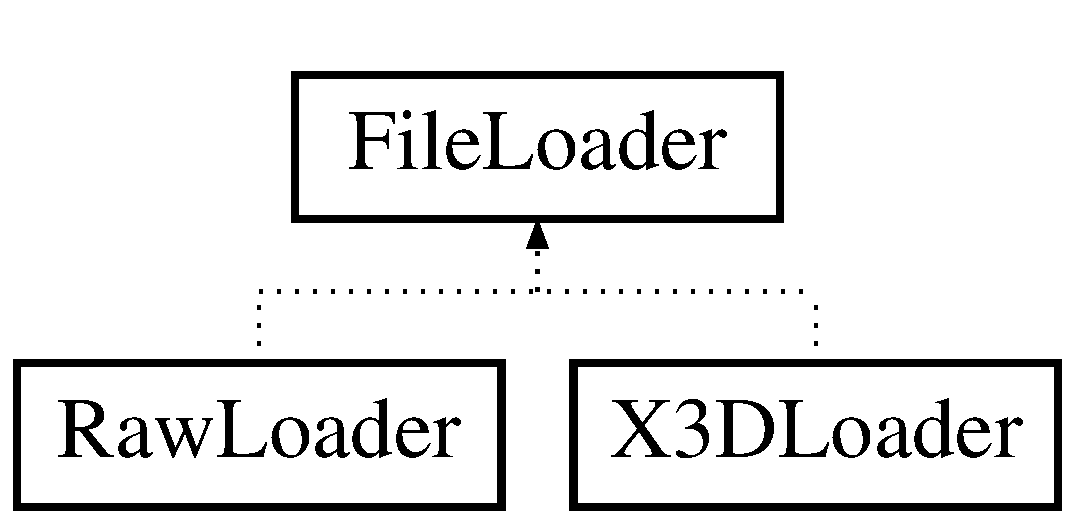
\includegraphics[height=2.000000cm]{classFileLoader}
\end{center}
\end{figure}
\subsection*{Static Public Member Functions}
\begin{DoxyCompactItemize}
\item 
static \hyperlink{classScene}{Scene} $\ast$ \hyperlink{classFileLoader_aa10ddbcfa87213ec2d2ade5a51f4cbe0}{loadFile} (std::string path)  throw ( std::string )
\item 
static int \hyperlink{classFileLoader_a9586cbf540f225cc16a9fc90e22edad9}{checkFileExtension} (std::string path)
\item 
static int \hyperlink{classFileLoader_a32bc1a5954be88d3df694b106aff7e83}{getFileExtensionCode} (std::string path)
\end{DoxyCompactItemize}


\subsection{Member Function Documentation}
\hypertarget{classFileLoader_a9586cbf540f225cc16a9fc90e22edad9}{
\index{FileLoader@{FileLoader}!checkFileExtension@{checkFileExtension}}
\index{checkFileExtension@{checkFileExtension}!FileLoader@{FileLoader}}
\subsubsection[{checkFileExtension}]{\setlength{\rightskip}{0pt plus 5cm}int FileLoader::checkFileExtension (
\begin{DoxyParamCaption}
\item[{std::string}]{path}
\end{DoxyParamCaption}
)\hspace{0.3cm}{\ttfamily  \mbox{[}static\mbox{]}}}}
\label{classFileLoader_a9586cbf540f225cc16a9fc90e22edad9}
Checks if the specified file has a valid file extension \begin{DoxyReturn}{Returns}
an int representing which file extension was present, if a unknown file extension was present return -\/1. 
\end{DoxyReturn}
\hypertarget{classFileLoader_a32bc1a5954be88d3df694b106aff7e83}{
\index{FileLoader@{FileLoader}!getFileExtensionCode@{getFileExtensionCode}}
\index{getFileExtensionCode@{getFileExtensionCode}!FileLoader@{FileLoader}}
\subsubsection[{getFileExtensionCode}]{\setlength{\rightskip}{0pt plus 5cm}int FileLoader::getFileExtensionCode (
\begin{DoxyParamCaption}
\item[{std::string}]{fileExtension}
\end{DoxyParamCaption}
)\hspace{0.3cm}{\ttfamily  \mbox{[}static\mbox{]}}}}
\label{classFileLoader_a32bc1a5954be88d3df694b106aff7e83}
Get the code representing the file extension 
\begin{DoxyParams}{Parameters}
{\em fileExtension} & will be compared internally with known file extensions \\
\hline
\end{DoxyParams}
\begin{DoxyReturn}{Returns}
an int representing which file extension was present, if a unknown file extension was present return -\/1. 
\end{DoxyReturn}
\hypertarget{classFileLoader_aa10ddbcfa87213ec2d2ade5a51f4cbe0}{
\index{FileLoader@{FileLoader}!loadFile@{loadFile}}
\index{loadFile@{loadFile}!FileLoader@{FileLoader}}
\subsubsection[{loadFile}]{\setlength{\rightskip}{0pt plus 5cm}{\bf Scene} $\ast$ FileLoader::loadFile (
\begin{DoxyParamCaption}
\item[{std::string}]{path}
\end{DoxyParamCaption}
)  throw ( std::string )\hspace{0.3cm}{\ttfamily  \mbox{[}static\mbox{]}}}}
\label{classFileLoader_aa10ddbcfa87213ec2d2ade5a51f4cbe0}
Loads a file, and from which creates a \hyperlink{classScene}{Scene} object. 
\begin{DoxyParams}{Parameters}
{\em path} & the filepath to load a file from \\
\hline
\end{DoxyParams}
\begin{DoxyReturn}{Returns}
A \hyperlink{classScene}{Scene} containing the contents acquired from the specified file 
\end{DoxyReturn}


Reimplemented in \hyperlink{classRawLoader_a9c9f9267310cc3f707482b818011dbdb}{RawLoader}, and \hyperlink{classX3DLoader_a2693e6c06a6d60e13321e8d9155cc31c}{X3DLoader}.



The documentation for this class was generated from the following files:\begin{DoxyCompactItemize}
\item 
FileLoader.h\item 
FileLoader.cpp\end{DoxyCompactItemize}

\hypertarget{classGraphicalObject}{
\section{GraphicalObject Class Reference}
\label{classGraphicalObject}\index{GraphicalObject@{GraphicalObject}}
}
\subsection*{Public Member Functions}
\begin{DoxyCompactItemize}
\item 
\hypertarget{classGraphicalObject_ae30831806efa43bde19640c8857559ce}{
{\bfseries GraphicalObject} (float vertexData\mbox{[}$\,$\mbox{]}, int size)}
\label{classGraphicalObject_ae30831806efa43bde19640c8857559ce}

\item 
\hyperlink{classGraphicalObject_ad0d5c734f217597805c0a3791130c6b4}{GraphicalObject} (float vertexData\mbox{[}$\,$\mbox{]}, int vertexDatasSize, float colorData\mbox{[}$\,$\mbox{]}, int ColorDataSize)
\item 
float $\ast$ \hyperlink{classGraphicalObject_a97f317570e78a61e753ae184c76eec29}{getVertexData} ()
\item 
float $\ast$ \hyperlink{classGraphicalObject_a50a8d9619867bfb406c9bdc613da8c7a}{getColorData} ()
\item 
int \hyperlink{classGraphicalObject_a3af39e1e523f9cf1405c02ddbc10cae6}{getVertexDataSize} ()
\item 
int \hyperlink{classGraphicalObject_a06aaea6903c56f878c5621ad64464603}{getColorDataSize} ()
\item 
void \hyperlink{classGraphicalObject_a4b5f37bd0b3ac26416ba186ce8a363dd}{bindBufferData} ()
\item 
void \hyperlink{classGraphicalObject_a78ddb331c286a2b749094b05dfbf3a8f}{draw} ()
\item 
void \hyperlink{classGraphicalObject_a4da3f17543b491a807049e60026586a6}{setOrigin} (\hyperlink{structVec3}{Vec3} ori)
\item 
\hyperlink{structVec3}{Vec3} \hyperlink{classGraphicalObject_a70c1917879aeb88cd640c01793ac0bbd}{getOrigin} ()
\item 
void \hyperlink{classGraphicalObject_ac07d03dbd89f6b39ac3b0c97ba138583}{setColorTriangle} (int index, \hyperlink{structVec3Int}{Vec3Int} color)
\item 
void \hyperlink{classGraphicalObject_a9a702570748c867e8717b55d01abcd46}{rotateX} (float angle)
\item 
void \hyperlink{classGraphicalObject_ae2179d2934799c4e7ac8166e6be9a073}{rotateY} (float angle)
\item 
void \hyperlink{classGraphicalObject_a2620d1eac3a41cbb6b0f3dc0bb6b6335}{rotateZ} (float angle)
\item 
void \hyperlink{classGraphicalObject_a0f07f4a577b33f7ece14792fb1d2f99c}{setUniforms} (GLuint shader)
\item 
void \hyperlink{classGraphicalObject_a501ee793d689c1474cf9b5d3ca46b356}{resize} (double factor)
\item 
void \hyperlink{classGraphicalObject_ab39c8a59da860bcfe56d42aac140e879}{setHighlightUniform} (GLuint shader)
\item 
void \hyperlink{classGraphicalObject_aa3541351751ba02f0a370412eb940925}{toggleHighlight} ()
\item 
void \hyperlink{classGraphicalObject_abc3ff1ef131db3b36c40ae04d533daa3}{setHighlight} (bool \_\-bool)
\item 
void \hyperlink{classGraphicalObject_a304ff62328d4ced89fbb88951ca2f355}{setScale} (double \_\-scale)
\item 
double \hyperlink{classGraphicalObject_a266b270672c4da50c47bbd4cee7008e8}{getScale} ()
\item 
void \hyperlink{classGraphicalObject_a2d01a90fa8d7aa54a02e07d9e33eb993}{incrementScale} (double inc)
\item 
void \hyperlink{classGraphicalObject_a6582fd399673a5bd5dfcdbad00ff1966}{translate} (\hyperlink{structVec3}{Vec3} trans)
\item 
bool \hyperlink{classGraphicalObject_a99b117674c1de60cac36eadd5be3ff3f}{hasMesh} ()
\item 
\hypertarget{classGraphicalObject_acc1ff1412cf90e11b323bc0396f80534}{
bool {\bfseries highlighted} ()}
\label{classGraphicalObject_acc1ff1412cf90e11b323bc0396f80534}

\item 
void \hyperlink{classGraphicalObject_a499bbe0e9c9bc5bcff08465f97b60776}{setMesh} (bool mesh)
\item 
\hypertarget{classGraphicalObject_a13bf38db47440924c2cfa2eae0bbde07}{
void {\bfseries setPosition} (\hyperlink{structVec3}{Vec3} pos)}
\label{classGraphicalObject_a13bf38db47440924c2cfa2eae0bbde07}

\item 
\hypertarget{classGraphicalObject_a12144c8a86ff8b531d6caeae19f95ea4}{
\hyperlink{structVec3}{Vec3} {\bfseries getPosition} ()}
\label{classGraphicalObject_a12144c8a86ff8b531d6caeae19f95ea4}

\item 
void \hyperlink{classGraphicalObject_abd9b4745450b888e825420c534a7555f}{center} (\hyperlink{structVec3}{Vec3} camPos, \hyperlink{structVec3}{Vec3} optPos)
\end{DoxyCompactItemize}
\subsection*{Public Attributes}
\begin{DoxyCompactItemize}
\item 
\hypertarget{classGraphicalObject_a78331fe745cd3eb10ed1d10594cc2293}{
\hyperlink{structVec3}{Vec3} {\bfseries origin}}
\label{classGraphicalObject_a78331fe745cd3eb10ed1d10594cc2293}

\end{DoxyCompactItemize}


\subsection{Constructor \& Destructor Documentation}
\hypertarget{classGraphicalObject_ad0d5c734f217597805c0a3791130c6b4}{
\index{GraphicalObject@{GraphicalObject}!GraphicalObject@{GraphicalObject}}
\index{GraphicalObject@{GraphicalObject}!GraphicalObject@{GraphicalObject}}
\subsubsection[{GraphicalObject}]{\setlength{\rightskip}{0pt plus 5cm}GraphicalObject::GraphicalObject (
\begin{DoxyParamCaption}
\item[{float}]{\_\-vertexData\mbox{[}$\,$\mbox{]}, }
\item[{int}]{\_\-vertexDataSize, }
\item[{float}]{\_\-colorData\mbox{[}$\,$\mbox{]}, }
\item[{int}]{\_\-colorDataSize}
\end{DoxyParamCaption}
)}}
\label{classGraphicalObject_ad0d5c734f217597805c0a3791130c6b4}
\hyperlink{classGraphicalObject}{GraphicalObject} constructor 
\begin{DoxyParams}{Parameters}
{\em \_\-vertexData} & Array containing the vertex data. \\
\hline
{\em \_\-vertexDataSize} & Should be the number of floats in \_\-vertexData. \\
\hline
{\em \_\-colorData} & Array containing the color data for the object. \\
\hline
{\em \_\-colorDataSize} & Should be the number of floats in \_\-colorData. In most cases is \_\-colorDataSize = \_\-vertexDataSize. \\
\hline
\end{DoxyParams}


\subsection{Member Function Documentation}
\hypertarget{classGraphicalObject_a4b5f37bd0b3ac26416ba186ce8a363dd}{
\index{GraphicalObject@{GraphicalObject}!bindBufferData@{bindBufferData}}
\index{bindBufferData@{bindBufferData}!GraphicalObject@{GraphicalObject}}
\subsubsection[{bindBufferData}]{\setlength{\rightskip}{0pt plus 5cm}void GraphicalObject::bindBufferData (
\begin{DoxyParamCaption}
{}
\end{DoxyParamCaption}
)}}
\label{classGraphicalObject_a4b5f37bd0b3ac26416ba186ce8a363dd}
Binds the buffer data of colarData and vertexData. Must be done before calling the method \hyperlink{classGraphicalObject_a78ddb331c286a2b749094b05dfbf3a8f}{draw()}. \hypertarget{classGraphicalObject_abd9b4745450b888e825420c534a7555f}{
\index{GraphicalObject@{GraphicalObject}!center@{center}}
\index{center@{center}!GraphicalObject@{GraphicalObject}}
\subsubsection[{center}]{\setlength{\rightskip}{0pt plus 5cm}void GraphicalObject::center (
\begin{DoxyParamCaption}
\item[{{\bf Vec3}}]{camPos, }
\item[{{\bf Vec3}}]{optPos}
\end{DoxyParamCaption}
)}}
\label{classGraphicalObject_abd9b4745450b888e825420c534a7555f}
Tries to center the object around the given position. Relative to the cameras position. Does not take rotation into account. 
\begin{DoxyParams}{Parameters}
{\em camPos} & The cameras offset. \\
\hline
{\em optPos} & The point in space where the object will be centered around. \\
\hline
\end{DoxyParams}
\hypertarget{classGraphicalObject_a78ddb331c286a2b749094b05dfbf3a8f}{
\index{GraphicalObject@{GraphicalObject}!draw@{draw}}
\index{draw@{draw}!GraphicalObject@{GraphicalObject}}
\subsubsection[{draw}]{\setlength{\rightskip}{0pt plus 5cm}void GraphicalObject::draw (
\begin{DoxyParamCaption}
{}
\end{DoxyParamCaption}
)}}
\label{classGraphicalObject_a78ddb331c286a2b749094b05dfbf3a8f}
Draws the object. \hypertarget{classGraphicalObject_a50a8d9619867bfb406c9bdc613da8c7a}{
\index{GraphicalObject@{GraphicalObject}!getColorData@{getColorData}}
\index{getColorData@{getColorData}!GraphicalObject@{GraphicalObject}}
\subsubsection[{getColorData}]{\setlength{\rightskip}{0pt plus 5cm}float $\ast$ GraphicalObject::getColorData (
\begin{DoxyParamCaption}
{}
\end{DoxyParamCaption}
)}}
\label{classGraphicalObject_a50a8d9619867bfb406c9bdc613da8c7a}
Returns the objects color data array. \begin{DoxyReturn}{Returns}
Objects color data array. 
\end{DoxyReturn}
\hypertarget{classGraphicalObject_a06aaea6903c56f878c5621ad64464603}{
\index{GraphicalObject@{GraphicalObject}!getColorDataSize@{getColorDataSize}}
\index{getColorDataSize@{getColorDataSize}!GraphicalObject@{GraphicalObject}}
\subsubsection[{getColorDataSize}]{\setlength{\rightskip}{0pt plus 5cm}int GraphicalObject::getColorDataSize (
\begin{DoxyParamCaption}
{}
\end{DoxyParamCaption}
)}}
\label{classGraphicalObject_a06aaea6903c56f878c5621ad64464603}
Returns the color data array size. \begin{DoxyReturn}{Returns}
Color data array size. 
\end{DoxyReturn}
\hypertarget{classGraphicalObject_a70c1917879aeb88cd640c01793ac0bbd}{
\index{GraphicalObject@{GraphicalObject}!getOrigin@{getOrigin}}
\index{getOrigin@{getOrigin}!GraphicalObject@{GraphicalObject}}
\subsubsection[{getOrigin}]{\setlength{\rightskip}{0pt plus 5cm}{\bf Vec3} GraphicalObject::getOrigin (
\begin{DoxyParamCaption}
{}
\end{DoxyParamCaption}
)}}
\label{classGraphicalObject_a70c1917879aeb88cd640c01793ac0bbd}
Get the objects origin \begin{DoxyReturn}{Returns}
the object origin 
\end{DoxyReturn}
\hypertarget{classGraphicalObject_a266b270672c4da50c47bbd4cee7008e8}{
\index{GraphicalObject@{GraphicalObject}!getScale@{getScale}}
\index{getScale@{getScale}!GraphicalObject@{GraphicalObject}}
\subsubsection[{getScale}]{\setlength{\rightskip}{0pt plus 5cm}double GraphicalObject::getScale (
\begin{DoxyParamCaption}
{}
\end{DoxyParamCaption}
)}}
\label{classGraphicalObject_a266b270672c4da50c47bbd4cee7008e8}
Returns the scale of the object. \begin{DoxyReturn}{Returns}
The scale. 
\end{DoxyReturn}
\hypertarget{classGraphicalObject_a97f317570e78a61e753ae184c76eec29}{
\index{GraphicalObject@{GraphicalObject}!getVertexData@{getVertexData}}
\index{getVertexData@{getVertexData}!GraphicalObject@{GraphicalObject}}
\subsubsection[{getVertexData}]{\setlength{\rightskip}{0pt plus 5cm}float $\ast$ GraphicalObject::getVertexData (
\begin{DoxyParamCaption}
{}
\end{DoxyParamCaption}
)}}
\label{classGraphicalObject_a97f317570e78a61e753ae184c76eec29}
Returns the objects vertex data array. \begin{DoxyReturn}{Returns}
Objects vertex data array. 
\end{DoxyReturn}
\hypertarget{classGraphicalObject_a3af39e1e523f9cf1405c02ddbc10cae6}{
\index{GraphicalObject@{GraphicalObject}!getVertexDataSize@{getVertexDataSize}}
\index{getVertexDataSize@{getVertexDataSize}!GraphicalObject@{GraphicalObject}}
\subsubsection[{getVertexDataSize}]{\setlength{\rightskip}{0pt plus 5cm}int GraphicalObject::getVertexDataSize (
\begin{DoxyParamCaption}
{}
\end{DoxyParamCaption}
)}}
\label{classGraphicalObject_a3af39e1e523f9cf1405c02ddbc10cae6}
Returns the color data vertex size. \begin{DoxyReturn}{Returns}
Color data vertex size. 
\end{DoxyReturn}
\hypertarget{classGraphicalObject_a99b117674c1de60cac36eadd5be3ff3f}{
\index{GraphicalObject@{GraphicalObject}!hasMesh@{hasMesh}}
\index{hasMesh@{hasMesh}!GraphicalObject@{GraphicalObject}}
\subsubsection[{hasMesh}]{\setlength{\rightskip}{0pt plus 5cm}bool GraphicalObject::hasMesh (
\begin{DoxyParamCaption}
{}
\end{DoxyParamCaption}
)}}
\label{classGraphicalObject_a99b117674c1de60cac36eadd5be3ff3f}
Checks if the object is meshed. \begin{DoxyReturn}{Returns}
True if the object is meshed. False otherwise. 
\end{DoxyReturn}
\hypertarget{classGraphicalObject_a2d01a90fa8d7aa54a02e07d9e33eb993}{
\index{GraphicalObject@{GraphicalObject}!incrementScale@{incrementScale}}
\index{incrementScale@{incrementScale}!GraphicalObject@{GraphicalObject}}
\subsubsection[{incrementScale}]{\setlength{\rightskip}{0pt plus 5cm}void GraphicalObject::incrementScale (
\begin{DoxyParamCaption}
\item[{double}]{inc}
\end{DoxyParamCaption}
)}}
\label{classGraphicalObject_a2d01a90fa8d7aa54a02e07d9e33eb993}
Increments the objects scale. 
\begin{DoxyParams}{Parameters}
{\em inc} & The increment. \\
\hline
\end{DoxyParams}
\hypertarget{classGraphicalObject_a501ee793d689c1474cf9b5d3ca46b356}{
\index{GraphicalObject@{GraphicalObject}!resize@{resize}}
\index{resize@{resize}!GraphicalObject@{GraphicalObject}}
\subsubsection[{resize}]{\setlength{\rightskip}{0pt plus 5cm}void GraphicalObject::resize (
\begin{DoxyParamCaption}
\item[{double}]{factor}
\end{DoxyParamCaption}
)}}
\label{classGraphicalObject_a501ee793d689c1474cf9b5d3ca46b356}
Scales the object by the provided factor. 
\begin{DoxyParams}{Parameters}
{\em factor} & The factor for scaling. \\
\hline
\end{DoxyParams}
\hypertarget{classGraphicalObject_a9a702570748c867e8717b55d01abcd46}{
\index{GraphicalObject@{GraphicalObject}!rotateX@{rotateX}}
\index{rotateX@{rotateX}!GraphicalObject@{GraphicalObject}}
\subsubsection[{rotateX}]{\setlength{\rightskip}{0pt plus 5cm}void GraphicalObject::rotateX (
\begin{DoxyParamCaption}
\item[{float}]{angle}
\end{DoxyParamCaption}
)}}
\label{classGraphicalObject_a9a702570748c867e8717b55d01abcd46}
Rotate the x angle in radians and calculate the rotation. 
\begin{DoxyParams}{Parameters}
{\em angle} & Angular adjustment. \\
\hline
\end{DoxyParams}
\hypertarget{classGraphicalObject_ae2179d2934799c4e7ac8166e6be9a073}{
\index{GraphicalObject@{GraphicalObject}!rotateY@{rotateY}}
\index{rotateY@{rotateY}!GraphicalObject@{GraphicalObject}}
\subsubsection[{rotateY}]{\setlength{\rightskip}{0pt plus 5cm}void GraphicalObject::rotateY (
\begin{DoxyParamCaption}
\item[{float}]{angle}
\end{DoxyParamCaption}
)}}
\label{classGraphicalObject_ae2179d2934799c4e7ac8166e6be9a073}
Rotate the y angle in radians and calculate the rotation. 
\begin{DoxyParams}{Parameters}
{\em angle} & Angular adjustment. \\
\hline
\end{DoxyParams}
\hypertarget{classGraphicalObject_a2620d1eac3a41cbb6b0f3dc0bb6b6335}{
\index{GraphicalObject@{GraphicalObject}!rotateZ@{rotateZ}}
\index{rotateZ@{rotateZ}!GraphicalObject@{GraphicalObject}}
\subsubsection[{rotateZ}]{\setlength{\rightskip}{0pt plus 5cm}void GraphicalObject::rotateZ (
\begin{DoxyParamCaption}
\item[{float}]{angle}
\end{DoxyParamCaption}
)}}
\label{classGraphicalObject_a2620d1eac3a41cbb6b0f3dc0bb6b6335}
Rotate the z angle in radians and calculate the rotation. 
\begin{DoxyParams}{Parameters}
{\em angle} & Angular adjustment. \\
\hline
\end{DoxyParams}
\hypertarget{classGraphicalObject_ac07d03dbd89f6b39ac3b0c97ba138583}{
\index{GraphicalObject@{GraphicalObject}!setColorTriangle@{setColorTriangle}}
\index{setColorTriangle@{setColorTriangle}!GraphicalObject@{GraphicalObject}}
\subsubsection[{setColorTriangle}]{\setlength{\rightskip}{0pt plus 5cm}void GraphicalObject::setColorTriangle (
\begin{DoxyParamCaption}
\item[{int}]{index, }
\item[{{\bf Vec3Int}}]{color}
\end{DoxyParamCaption}
)}}
\label{classGraphicalObject_ac07d03dbd89f6b39ac3b0c97ba138583}
Sets a triangle at an index to the specified color 
\begin{DoxyParams}{Parameters}
{\em index} & is the index of the triangle to change color on \\
\hline
{\em color} & is a 3 int vector taking a value between 0 255 for each component invalid values will be set to zero \\
\hline
\end{DoxyParams}
\hypertarget{classGraphicalObject_abc3ff1ef131db3b36c40ae04d533daa3}{
\index{GraphicalObject@{GraphicalObject}!setHighlight@{setHighlight}}
\index{setHighlight@{setHighlight}!GraphicalObject@{GraphicalObject}}
\subsubsection[{setHighlight}]{\setlength{\rightskip}{0pt plus 5cm}void GraphicalObject::setHighlight (
\begin{DoxyParamCaption}
\item[{bool}]{\_\-bool}
\end{DoxyParamCaption}
)}}
\label{classGraphicalObject_abc3ff1ef131db3b36c40ae04d533daa3}
Sets the highlight boolean. 
\begin{DoxyParams}{Parameters}
{\em \_\-bool} & The new highlight value. \\
\hline
\end{DoxyParams}
\hypertarget{classGraphicalObject_ab39c8a59da860bcfe56d42aac140e879}{
\index{GraphicalObject@{GraphicalObject}!setHighlightUniform@{setHighlightUniform}}
\index{setHighlightUniform@{setHighlightUniform}!GraphicalObject@{GraphicalObject}}
\subsubsection[{setHighlightUniform}]{\setlength{\rightskip}{0pt plus 5cm}void GraphicalObject::setHighlightUniform (
\begin{DoxyParamCaption}
\item[{GLuint}]{shader}
\end{DoxyParamCaption}
)}}
\label{classGraphicalObject_ab39c8a59da860bcfe56d42aac140e879}
Sets the highlight uniform so it can be accessed by the shader. 
\begin{DoxyParams}{Parameters}
{\em shader} & The shader that uses the highlight uniform. \\
\hline
\end{DoxyParams}
\hypertarget{classGraphicalObject_a499bbe0e9c9bc5bcff08465f97b60776}{
\index{GraphicalObject@{GraphicalObject}!setMesh@{setMesh}}
\index{setMesh@{setMesh}!GraphicalObject@{GraphicalObject}}
\subsubsection[{setMesh}]{\setlength{\rightskip}{0pt plus 5cm}void GraphicalObject::setMesh (
\begin{DoxyParamCaption}
\item[{bool}]{\_\-mesh}
\end{DoxyParamCaption}
)}}
\label{classGraphicalObject_a499bbe0e9c9bc5bcff08465f97b60776}
Sets mesh to TRUE or FALSE. 
\begin{DoxyParams}{Parameters}
{\em \_\-mesh} & The new mesh boolean. \\
\hline
\end{DoxyParams}
\hypertarget{classGraphicalObject_a4da3f17543b491a807049e60026586a6}{
\index{GraphicalObject@{GraphicalObject}!setOrigin@{setOrigin}}
\index{setOrigin@{setOrigin}!GraphicalObject@{GraphicalObject}}
\subsubsection[{setOrigin}]{\setlength{\rightskip}{0pt plus 5cm}void GraphicalObject::setOrigin (
\begin{DoxyParamCaption}
\item[{{\bf Vec3}}]{ori}
\end{DoxyParamCaption}
)}}
\label{classGraphicalObject_a4da3f17543b491a807049e60026586a6}
Sets the origin for the object. The origin is the point in space which the object will rotate around. 
\begin{DoxyParams}{Parameters}
{\em ori} & The new origin value. \\
\hline
\end{DoxyParams}
\hypertarget{classGraphicalObject_a304ff62328d4ced89fbb88951ca2f355}{
\index{GraphicalObject@{GraphicalObject}!setScale@{setScale}}
\index{setScale@{setScale}!GraphicalObject@{GraphicalObject}}
\subsubsection[{setScale}]{\setlength{\rightskip}{0pt plus 5cm}void GraphicalObject::setScale (
\begin{DoxyParamCaption}
\item[{double}]{\_\-scale}
\end{DoxyParamCaption}
)}}
\label{classGraphicalObject_a304ff62328d4ced89fbb88951ca2f355}
Sets the scale of the object. 
\begin{DoxyParams}{Parameters}
{\em \_\-scala} & The scale. \\
\hline
\end{DoxyParams}
\hypertarget{classGraphicalObject_a0f07f4a577b33f7ece14792fb1d2f99c}{
\index{GraphicalObject@{GraphicalObject}!setUniforms@{setUniforms}}
\index{setUniforms@{setUniforms}!GraphicalObject@{GraphicalObject}}
\subsubsection[{setUniforms}]{\setlength{\rightskip}{0pt plus 5cm}void GraphicalObject::setUniforms (
\begin{DoxyParamCaption}
\item[{GLuint}]{shader}
\end{DoxyParamCaption}
)}}
\label{classGraphicalObject_a0f07f4a577b33f7ece14792fb1d2f99c}
Sets the scale, objectRot, objectPos and objOrigin uniforms so they can be accessed by the shader. 
\begin{DoxyParams}{Parameters}
{\em shader} & The shader that uses the scale, objectRot, objectPos and objOrigin uniforms. \\
\hline
\end{DoxyParams}
\hypertarget{classGraphicalObject_aa3541351751ba02f0a370412eb940925}{
\index{GraphicalObject@{GraphicalObject}!toggleHighlight@{toggleHighlight}}
\index{toggleHighlight@{toggleHighlight}!GraphicalObject@{GraphicalObject}}
\subsubsection[{toggleHighlight}]{\setlength{\rightskip}{0pt plus 5cm}void GraphicalObject::toggleHighlight (
\begin{DoxyParamCaption}
{}
\end{DoxyParamCaption}
)}}
\label{classGraphicalObject_aa3541351751ba02f0a370412eb940925}
Toggles the highligh boolean. If highlight = TRUE before the call to \hyperlink{classGraphicalObject_aa3541351751ba02f0a370412eb940925}{toggleHighlight()} it will be FALSE after and vise versa. \hypertarget{classGraphicalObject_a6582fd399673a5bd5dfcdbad00ff1966}{
\index{GraphicalObject@{GraphicalObject}!translate@{translate}}
\index{translate@{translate}!GraphicalObject@{GraphicalObject}}
\subsubsection[{translate}]{\setlength{\rightskip}{0pt plus 5cm}void GraphicalObject::translate (
\begin{DoxyParamCaption}
\item[{{\bf Vec3}}]{trans}
\end{DoxyParamCaption}
)}}
\label{classGraphicalObject_a6582fd399673a5bd5dfcdbad00ff1966}
Translates the object by the given offset by updating the pos variable. 
\begin{DoxyParams}{Parameters}
{\em trans} & A \hyperlink{structVec3}{Vec3} containing the offset values. \\
\hline
\end{DoxyParams}


The documentation for this class was generated from the following files:\begin{DoxyCompactItemize}
\item 
GraphicalObject.h\item 
GraphicalObject.cpp\end{DoxyCompactItemize}

\hypertarget{structKeystoneSetting}{
\section{KeystoneSetting Struct Reference}
\label{structKeystoneSetting}\index{KeystoneSetting@{KeystoneSetting}}
}
\subsection*{Public Attributes}
\begin{DoxyCompactItemize}
\item 
\hypertarget{structKeystoneSetting_af5d1739dd1cf1a477cd4b92bf138f5de}{
float {\bfseries k} \mbox{[}8\mbox{]}}
\label{structKeystoneSetting_af5d1739dd1cf1a477cd4b92bf138f5de}

\end{DoxyCompactItemize}


The documentation for this struct was generated from the following file:\begin{DoxyCompactItemize}
\item 
Shared.h\end{DoxyCompactItemize}

\hypertarget{structMat4}{
\section{Mat4 Struct Reference}
\label{structMat4}\index{Mat4@{Mat4}}
}
\subsection*{Static Public Member Functions}
\begin{DoxyCompactItemize}
\item 
\hypertarget{structMat4_ab29a68f1742b080d5ca1a60f47dfaf83}{
static \hyperlink{structMat4}{Mat4} {\bfseries matrixMultiplication} (\hyperlink{structMat4}{Mat4} a, \hyperlink{structMat4}{Mat4} b)}
\label{structMat4_ab29a68f1742b080d5ca1a60f47dfaf83}

\end{DoxyCompactItemize}
\subsection*{Public Attributes}
\begin{DoxyCompactItemize}
\item 
\hypertarget{structMat4_ad475f9d364516e86058ed2784530a05d}{
float {\bfseries m} \mbox{[}16\mbox{]}}
\label{structMat4_ad475f9d364516e86058ed2784530a05d}

\end{DoxyCompactItemize}


The documentation for this struct was generated from the following file:\begin{DoxyCompactItemize}
\item 
Shared.h\end{DoxyCompactItemize}

\hypertarget{classMonitor}{
\section{Monitor Class Reference}
\label{classMonitor}\index{Monitor@{Monitor}}
}


{\ttfamily \#include $<$Monitor.h$>$}

\subsection*{Public Member Functions}
\begin{DoxyCompactItemize}
\item 
\hyperlink{classMonitor_a639d27b16055d8681c2015d00ea083d8}{Monitor} ()
\item 
\hyperlink{classMonitor_a64aba8195effc068092ddea5a71e8176}{$\sim$Monitor} ()
\item 
void \hyperlink{classMonitor_adb084d156c6e01816a4158dfe71c142f}{display} (\hyperlink{classScene}{Scene} scene)
\item 
void \hyperlink{classMonitor_a21b504df5c53c279e94178de182af854}{addShader} (\hyperlink{classShader}{Shader} shader)
\item 
std::vector$<$ \hyperlink{classShader}{Shader} $>$ \hyperlink{classMonitor_ab0df82e6f794c5f9910f2ea9c879adb2}{getShaders} ()
\item 
\hypertarget{classMonitor_a0080eb7efa685555ec8ac8d5218f75a1}{
\hyperlink{classProjector}{Projector} $\ast$ {\bfseries getProjector} ()}
\label{classMonitor_a0080eb7efa685555ec8ac8d5218f75a1}

\end{DoxyCompactItemize}


\subsection{Detailed Description}
\hyperlink{classMonitor}{Monitor} class. 

\subsection{Constructor \& Destructor Documentation}
\hypertarget{classMonitor_a639d27b16055d8681c2015d00ea083d8}{
\index{Monitor@{Monitor}!Monitor@{Monitor}}
\index{Monitor@{Monitor}!Monitor@{Monitor}}
\subsubsection[{Monitor}]{\setlength{\rightskip}{0pt plus 5cm}Monitor::Monitor (
\begin{DoxyParamCaption}
{}
\end{DoxyParamCaption}
)}}
\label{classMonitor_a639d27b16055d8681c2015d00ea083d8}
\hyperlink{classMonitor}{Monitor} constructor. \hypertarget{classMonitor_a64aba8195effc068092ddea5a71e8176}{
\index{Monitor@{Monitor}!$\sim$Monitor@{$\sim$Monitor}}
\index{$\sim$Monitor@{$\sim$Monitor}!Monitor@{Monitor}}
\subsubsection[{$\sim$Monitor}]{\setlength{\rightskip}{0pt plus 5cm}Monitor::$\sim$Monitor (
\begin{DoxyParamCaption}
{}
\end{DoxyParamCaption}
)}}
\label{classMonitor_a64aba8195effc068092ddea5a71e8176}
\hyperlink{classMonitor}{Monitor} destructor. 

\subsection{Member Function Documentation}
\hypertarget{classMonitor_a21b504df5c53c279e94178de182af854}{
\index{Monitor@{Monitor}!addShader@{addShader}}
\index{addShader@{addShader}!Monitor@{Monitor}}
\subsubsection[{addShader}]{\setlength{\rightskip}{0pt plus 5cm}void Monitor::addShader (
\begin{DoxyParamCaption}
\item[{{\bf Shader}}]{shader}
\end{DoxyParamCaption}
)}}
\label{classMonitor_a21b504df5c53c279e94178de182af854}
Adds a shader to rendering. 
\begin{DoxyParams}{Parameters}
{\em s} & \hyperlink{classShader}{Shader} to add. \\
\hline
\end{DoxyParams}
\hypertarget{classMonitor_adb084d156c6e01816a4158dfe71c142f}{
\index{Monitor@{Monitor}!display@{display}}
\index{display@{display}!Monitor@{Monitor}}
\subsubsection[{display}]{\setlength{\rightskip}{0pt plus 5cm}void Monitor::display (
\begin{DoxyParamCaption}
\item[{{\bf Scene}}]{scene}
\end{DoxyParamCaption}
)}}
\label{classMonitor_adb084d156c6e01816a4158dfe71c142f}
Displays a scene. 
\begin{DoxyParams}{Parameters}
{\em scn} & \hyperlink{classScene}{Scene} to display. \\
\hline
\end{DoxyParams}
\hypertarget{classMonitor_ab0df82e6f794c5f9910f2ea9c879adb2}{
\index{Monitor@{Monitor}!getShaders@{getShaders}}
\index{getShaders@{getShaders}!Monitor@{Monitor}}
\subsubsection[{getShaders}]{\setlength{\rightskip}{0pt plus 5cm}std::vector$<$ {\bf Shader} $>$ Monitor::getShaders (
\begin{DoxyParamCaption}
{}
\end{DoxyParamCaption}
)}}
\label{classMonitor_ab0df82e6f794c5f9910f2ea9c879adb2}
Returns a list of shaders. \begin{DoxyReturn}{Returns}
All associated shaders. 
\end{DoxyReturn}


The documentation for this class was generated from the following files:\begin{DoxyCompactItemize}
\item 
Monitor.h\item 
Monitor.cpp\end{DoxyCompactItemize}

\hypertarget{classProjector}{
\section{Projector Class Reference}
\label{classProjector}\index{Projector@{Projector}}
}
\subsection*{Public Member Functions}
\begin{DoxyCompactItemize}
\item 
\hyperlink{classProjector_ac3b7b98ff0014b2c94f1f0038381f78a}{Projector} (int $\ast$pointer, unsigned int len)
\item 
\hypertarget{classProjector_a81eb429cd0c4659149a563bf7aaba8f5}{
{\bfseries Projector} (\hyperlink{classConfiguration}{Configuration} $\ast$c)}
\label{classProjector_a81eb429cd0c4659149a563bf7aaba8f5}

\item 
\hyperlink{classProjector_a39d6c9ed1b6cb029aaf7df4586e6af8a}{Projector} (int $\ast$pointer, unsigned int len, \hyperlink{structVec3}{Vec3} pos, \hyperlink{structVec3}{Vec3} dir)
\item 
unsigned int \hyperlink{classProjector_a8714a339afd4da16f7949dfde0c30b0a}{getBufferSize} ()
\item 
\hyperlink{classColorTranslator}{ColorTranslator} $\ast$ \hyperlink{classProjector_aaf340dde1e1a590742200007e4aecd02}{getColorTranslator} ()
\item 
void \hyperlink{classProjector_a500a8dbee7f243014dc9e8487fee69db}{setConfiguration} (\hyperlink{classConfiguration}{Configuration} c)
\item 
\hyperlink{classConfiguration}{Configuration} \hyperlink{classProjector_a54417b48fb015e507628d5feb75bfccc}{getConfiguration} ()
\item 
void \hyperlink{classProjector_a81a631412be8114bde82a155eab5279a}{highlight} ()
\item 
void \hyperlink{classProjector_acf0914f15c887e09aef49a7c13a5e1cd}{unHighlight} ()
\item 
\hypertarget{classProjector_afcf269fbc38d9c73188aefedf4010e09}{
int $\ast$ {\bfseries getBuffer} ()}
\label{classProjector_afcf269fbc38d9c73188aefedf4010e09}

\item 
void \hyperlink{classProjector_a6ea6b55198d6fdfdf7b28c612e95ec26}{calcKeystone} (GLuint pid)  throw (std::string)
\item 
void \hyperlink{classProjector_a6e2ac751c6dafa3048eb25359ed0cd05}{display} (\hyperlink{classScene}{Scene} scene)
\item 
void \hyperlink{classProjector_a6dfc533175a56a0bf2989b5c0c917a36}{addShader} (\hyperlink{classShader}{Shader} shader)
\item 
std::vector$<$ \hyperlink{classShader}{Shader} $>$ \hyperlink{classProjector_ae356e74b51ffa74a9915b71825b2a774}{getShaders} ()
\item 
\hyperlink{structVec3}{Vec3} \hyperlink{classProjector_a68c643eead5cbe093e1c995c35d3a247}{getPosition} ()
\item 
\hyperlink{structVec3}{Vec3} \hyperlink{classProjector_a2094b745b60702602ab037d6485d030d}{getDirection} ()
\item 
void \hyperlink{classProjector_a8c606ce355da71accf80afe0ad8ab778}{setPosition} (\hyperlink{structVec3}{Vec3} position)
\item 
void \hyperlink{classProjector_a3bbcc7b641d3941cf347b3ce61fda7d6}{setDirection} (\hyperlink{structVec3}{Vec3} direction\_\-)
\item 
void \hyperlink{classProjector_af7fabc0089d4a6c961d473b009a3b50d}{moveKeystoneCorner} (int corner, int xory, float value)
\item 
void \hyperlink{classProjector_a47f7376f32cae68d15e35f4690351c50}{setKeystoneObserved} (\hyperlink{structKeystoneSetting}{KeystoneSetting} f)
\end{DoxyCompactItemize}


\subsection{Constructor \& Destructor Documentation}
\hypertarget{classProjector_ac3b7b98ff0014b2c94f1f0038381f78a}{
\index{Projector@{Projector}!Projector@{Projector}}
\index{Projector@{Projector}!Projector@{Projector}}
\subsubsection[{Projector}]{\setlength{\rightskip}{0pt plus 5cm}Projector::Projector (
\begin{DoxyParamCaption}
\item[{int $\ast$}]{pointer, }
\item[{unsigned int}]{len}
\end{DoxyParamCaption}
)}}
\label{classProjector_ac3b7b98ff0014b2c94f1f0038381f78a}
Creates a new projector with buffer of size len at the place pointer with position (0,0,0) and direction (0,0,0) 
\begin{DoxyParams}{Parameters}
{\em pointer} & Pointer to the rendering buffer. \\
\hline
{\em len} & Size of buffer in bytes. \\
\hline
\end{DoxyParams}
\hypertarget{classProjector_a39d6c9ed1b6cb029aaf7df4586e6af8a}{
\index{Projector@{Projector}!Projector@{Projector}}
\index{Projector@{Projector}!Projector@{Projector}}
\subsubsection[{Projector}]{\setlength{\rightskip}{0pt plus 5cm}Projector::Projector (
\begin{DoxyParamCaption}
\item[{int $\ast$}]{pointer, }
\item[{unsigned int}]{len, }
\item[{{\bf Vec3}}]{pos, }
\item[{{\bf Vec3}}]{dir}
\end{DoxyParamCaption}
)}}
\label{classProjector_a39d6c9ed1b6cb029aaf7df4586e6af8a}
Creates a new projector with a buffer of size len at the place pointer with position pos and direction dir 
\begin{DoxyParams}{Parameters}
{\em pointer} & Pointer to the rendering buffer. \\
\hline
{\em len} & Size of buffer in bytes. \\
\hline
{\em pos} & Position of the projector. \\
\hline
{\em dir} & Direction of the projector. \\
\hline
\end{DoxyParams}


\subsection{Member Function Documentation}
\hypertarget{classProjector_a6dfc533175a56a0bf2989b5c0c917a36}{
\index{Projector@{Projector}!addShader@{addShader}}
\index{addShader@{addShader}!Projector@{Projector}}
\subsubsection[{addShader}]{\setlength{\rightskip}{0pt plus 5cm}void Projector::addShader (
\begin{DoxyParamCaption}
\item[{{\bf Shader}}]{shader}
\end{DoxyParamCaption}
)}}
\label{classProjector_a6dfc533175a56a0bf2989b5c0c917a36}
Adds a shader object to the list of shaders. 
\begin{DoxyParams}{Parameters}
{\em shader} & the shader to add to the list. \\
\hline
\end{DoxyParams}
\hypertarget{classProjector_a6ea6b55198d6fdfdf7b28c612e95ec26}{
\index{Projector@{Projector}!calcKeystone@{calcKeystone}}
\index{calcKeystone@{calcKeystone}!Projector@{Projector}}
\subsubsection[{calcKeystone}]{\setlength{\rightskip}{0pt plus 5cm}void Projector::calcKeystone (
\begin{DoxyParamCaption}
\item[{GLuint}]{pid}
\end{DoxyParamCaption}
)  throw (std::string)}}
\label{classProjector_a6ea6b55198d6fdfdf7b28c612e95ec26}
Calculates the the keystone matrix and sets a uniform 
\begin{DoxyParams}{Parameters}
{\em pid} & is the shader program used when drawing \\
\hline
\end{DoxyParams}
\hypertarget{classProjector_a6e2ac751c6dafa3048eb25359ed0cd05}{
\index{Projector@{Projector}!display@{display}}
\index{display@{display}!Projector@{Projector}}
\subsubsection[{display}]{\setlength{\rightskip}{0pt plus 5cm}void Projector::display (
\begin{DoxyParamCaption}
\item[{{\bf Scene}}]{scene}
\end{DoxyParamCaption}
)}}
\label{classProjector_a6e2ac751c6dafa3048eb25359ed0cd05}
Displays the view through the projector associated with this instance. Prior to that it will also possibly have applied color settings and definitely applied keystone correction on the view. 
\begin{DoxyParams}{Parameters}
{\em takes} & a scene and draws in the current window \\
\hline
\end{DoxyParams}
\hypertarget{classProjector_a8714a339afd4da16f7949dfde0c30b0a}{
\index{Projector@{Projector}!getBufferSize@{getBufferSize}}
\index{getBufferSize@{getBufferSize}!Projector@{Projector}}
\subsubsection[{getBufferSize}]{\setlength{\rightskip}{0pt plus 5cm}unsigned int Projector::getBufferSize (
\begin{DoxyParamCaption}
{}
\end{DoxyParamCaption}
)}}
\label{classProjector_a8714a339afd4da16f7949dfde0c30b0a}
Returns the size of the buffer. \begin{DoxyReturn}{Returns}
Size of the buffer. 
\end{DoxyReturn}
\hypertarget{classProjector_aaf340dde1e1a590742200007e4aecd02}{
\index{Projector@{Projector}!getColorTranslator@{getColorTranslator}}
\index{getColorTranslator@{getColorTranslator}!Projector@{Projector}}
\subsubsection[{getColorTranslator}]{\setlength{\rightskip}{0pt plus 5cm}{\bf ColorTranslator} $\ast$ Projector::getColorTranslator (
\begin{DoxyParamCaption}
{}
\end{DoxyParamCaption}
)}}
\label{classProjector_aaf340dde1e1a590742200007e4aecd02}
Returns the associated colortranslator object. \begin{DoxyReturn}{Returns}
Colortranslator object. 
\end{DoxyReturn}
\hypertarget{classProjector_a54417b48fb015e507628d5feb75bfccc}{
\index{Projector@{Projector}!getConfiguration@{getConfiguration}}
\index{getConfiguration@{getConfiguration}!Projector@{Projector}}
\subsubsection[{getConfiguration}]{\setlength{\rightskip}{0pt plus 5cm}{\bf Configuration} Projector::getConfiguration (
\begin{DoxyParamCaption}
{}
\end{DoxyParamCaption}
)}}
\label{classProjector_a54417b48fb015e507628d5feb75bfccc}
Returns the current configuration. \begin{DoxyReturn}{Returns}
Current configuration. 
\end{DoxyReturn}
\hypertarget{classProjector_a2094b745b60702602ab037d6485d030d}{
\index{Projector@{Projector}!getDirection@{getDirection}}
\index{getDirection@{getDirection}!Projector@{Projector}}
\subsubsection[{getDirection}]{\setlength{\rightskip}{0pt plus 5cm}{\bf Vec3} Projector::getDirection (
\begin{DoxyParamCaption}
{}
\end{DoxyParamCaption}
)}}
\label{classProjector_a2094b745b60702602ab037d6485d030d}
Returns the direction of the projector as a \hyperlink{structVec3}{Vec3} object. \begin{DoxyReturn}{Returns}
the direction of the projector 
\end{DoxyReturn}
\hypertarget{classProjector_a68c643eead5cbe093e1c995c35d3a247}{
\index{Projector@{Projector}!getPosition@{getPosition}}
\index{getPosition@{getPosition}!Projector@{Projector}}
\subsubsection[{getPosition}]{\setlength{\rightskip}{0pt plus 5cm}{\bf Vec3} Projector::getPosition (
\begin{DoxyParamCaption}
{}
\end{DoxyParamCaption}
)}}
\label{classProjector_a68c643eead5cbe093e1c995c35d3a247}
Returns the position of the projector as a \hyperlink{structVec3}{Vec3} object. \begin{DoxyReturn}{Returns}
the position of the projector 
\end{DoxyReturn}
\hypertarget{classProjector_ae356e74b51ffa74a9915b71825b2a774}{
\index{Projector@{Projector}!getShaders@{getShaders}}
\index{getShaders@{getShaders}!Projector@{Projector}}
\subsubsection[{getShaders}]{\setlength{\rightskip}{0pt plus 5cm}std::vector$<$ {\bf Shader} $>$ Projector::getShaders (
\begin{DoxyParamCaption}
{}
\end{DoxyParamCaption}
)}}
\label{classProjector_ae356e74b51ffa74a9915b71825b2a774}
Gets the list of in use shaders. \begin{DoxyReturn}{Returns}
A list of shaders used by the projector 
\end{DoxyReturn}
\hypertarget{classProjector_a81a631412be8114bde82a155eab5279a}{
\index{Projector@{Projector}!highlight@{highlight}}
\index{highlight@{highlight}!Projector@{Projector}}
\subsubsection[{highlight}]{\setlength{\rightskip}{0pt plus 5cm}void Projector::highlight (
\begin{DoxyParamCaption}
{}
\end{DoxyParamCaption}
)}}
\label{classProjector_a81a631412be8114bde82a155eab5279a}
Highlights the background. \hypertarget{classProjector_af7fabc0089d4a6c961d473b009a3b50d}{
\index{Projector@{Projector}!moveKeystoneCorner@{moveKeystoneCorner}}
\index{moveKeystoneCorner@{moveKeystoneCorner}!Projector@{Projector}}
\subsubsection[{moveKeystoneCorner}]{\setlength{\rightskip}{0pt plus 5cm}void Projector::moveKeystoneCorner (
\begin{DoxyParamCaption}
\item[{int}]{corner, }
\item[{int}]{xory, }
\item[{float}]{value}
\end{DoxyParamCaption}
)}}
\label{classProjector_af7fabc0089d4a6c961d473b009a3b50d}
An interface to move the corners of the projected image, changing the observed values so that a new Keystone matrix can be calculated. 
\begin{DoxyParams}{Parameters}
{\em corner} & Which of the four coners to change \\
\hline
{\em xory} & States which component of the coordinate of a corner that should be changed X=0 Y=1 \\
\hline
{\em value} & Is the value to increase or decrease the component with \\
\hline
\end{DoxyParams}
\hypertarget{classProjector_a500a8dbee7f243014dc9e8487fee69db}{
\index{Projector@{Projector}!setConfiguration@{setConfiguration}}
\index{setConfiguration@{setConfiguration}!Projector@{Projector}}
\subsubsection[{setConfiguration}]{\setlength{\rightskip}{0pt plus 5cm}void Projector::setConfiguration (
\begin{DoxyParamCaption}
\item[{{\bf Configuration}}]{c}
\end{DoxyParamCaption}
)}}
\label{classProjector_a500a8dbee7f243014dc9e8487fee69db}
Set the current configuration. 
\begin{DoxyParams}{Parameters}
{\em c} & \hyperlink{classConfiguration}{Configuration} to be used. \\
\hline
\end{DoxyParams}
\hypertarget{classProjector_a3bbcc7b641d3941cf347b3ce61fda7d6}{
\index{Projector@{Projector}!setDirection@{setDirection}}
\index{setDirection@{setDirection}!Projector@{Projector}}
\subsubsection[{setDirection}]{\setlength{\rightskip}{0pt plus 5cm}void Projector::setDirection (
\begin{DoxyParamCaption}
\item[{{\bf Vec3}}]{\_\-direction}
\end{DoxyParamCaption}
)}}
\label{classProjector_a3bbcc7b641d3941cf347b3ce61fda7d6}
Sets the direction of the projectior to the parametre. 
\begin{DoxyParams}{Parameters}
{\em The} & new direction of the projector \\
\hline
\end{DoxyParams}
\hypertarget{classProjector_a47f7376f32cae68d15e35f4690351c50}{
\index{Projector@{Projector}!setKeystoneObserved@{setKeystoneObserved}}
\index{setKeystoneObserved@{setKeystoneObserved}!Projector@{Projector}}
\subsubsection[{setKeystoneObserved}]{\setlength{\rightskip}{0pt plus 5cm}void Projector::setKeystoneObserved (
\begin{DoxyParamCaption}
\item[{{\bf KeystoneSetting}}]{f}
\end{DoxyParamCaption}
)}}
\label{classProjector_a47f7376f32cae68d15e35f4690351c50}
Set the observed keystone values used when calculating the keystone matrix 
\begin{DoxyParams}{Parameters}
{\em f} & Is a \hyperlink{structKeystoneSetting}{KeystoneSetting} struct (contains 8 floats) \\
\hline
\end{DoxyParams}
\hypertarget{classProjector_a8c606ce355da71accf80afe0ad8ab778}{
\index{Projector@{Projector}!setPosition@{setPosition}}
\index{setPosition@{setPosition}!Projector@{Projector}}
\subsubsection[{setPosition}]{\setlength{\rightskip}{0pt plus 5cm}void Projector::setPosition (
\begin{DoxyParamCaption}
\item[{{\bf Vec3}}]{position}
\end{DoxyParamCaption}
)}}
\label{classProjector_a8c606ce355da71accf80afe0ad8ab778}
Sets the position of the projector to the value of the parametre. 
\begin{DoxyParams}{Parameters}
{\em The} & new position of the projector. \\
\hline
\end{DoxyParams}
\hypertarget{classProjector_acf0914f15c887e09aef49a7c13a5e1cd}{
\index{Projector@{Projector}!unHighlight@{unHighlight}}
\index{unHighlight@{unHighlight}!Projector@{Projector}}
\subsubsection[{unHighlight}]{\setlength{\rightskip}{0pt plus 5cm}void Projector::unHighlight (
\begin{DoxyParamCaption}
{}
\end{DoxyParamCaption}
)}}
\label{classProjector_acf0914f15c887e09aef49a7c13a5e1cd}
Disables highlighting of background. 

The documentation for this class was generated from the following files:\begin{DoxyCompactItemize}
\item 
Projector.h\item 
Projector.cpp\item 
real.cpp\end{DoxyCompactItemize}

\hypertarget{classRawLoader}{
\section{RawLoader Class Reference}
\label{classRawLoader}\index{RawLoader@{RawLoader}}
}
Inheritance diagram for RawLoader:\begin{figure}[H]
\begin{center}
\leavevmode
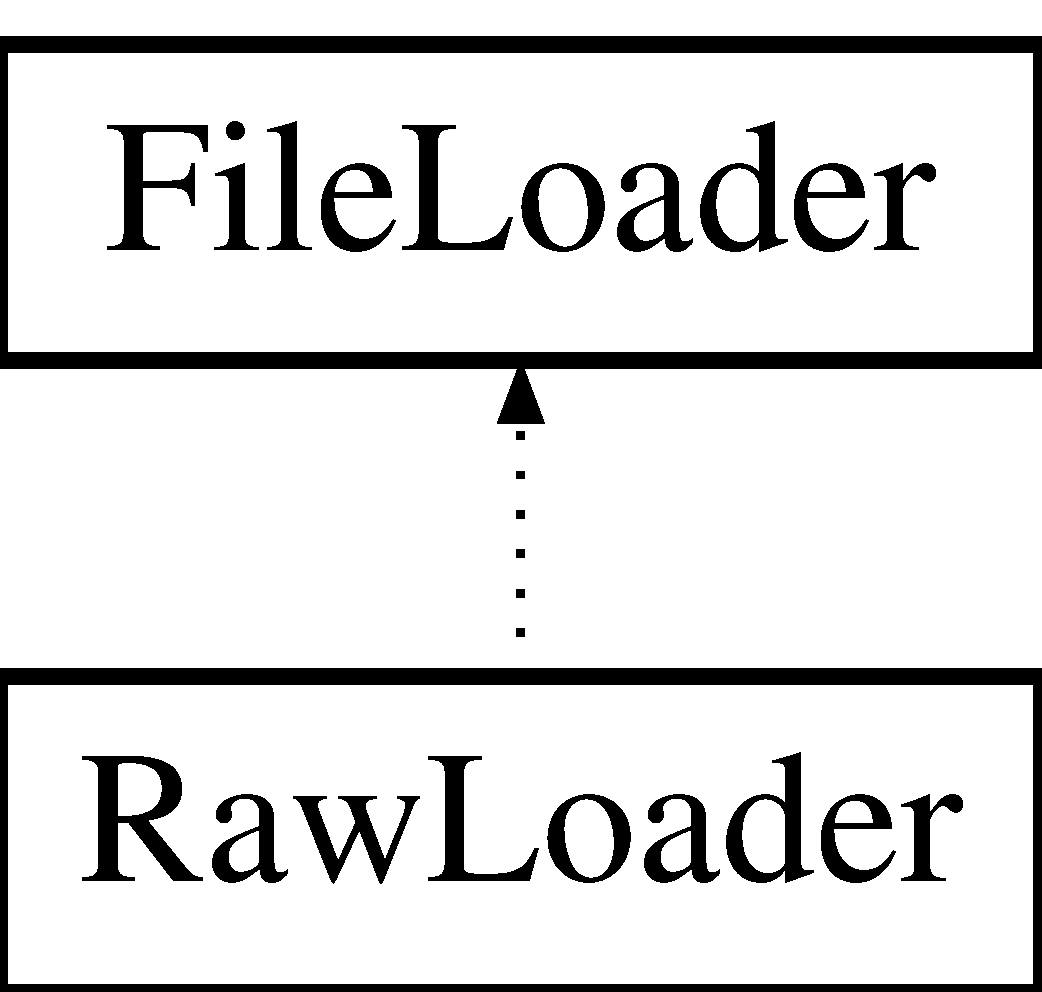
\includegraphics[height=2.000000cm]{classRawLoader}
\end{center}
\end{figure}
\subsection*{Static Public Member Functions}
\begin{DoxyCompactItemize}
\item 
static \hyperlink{classScene}{Scene} $\ast$ \hyperlink{classRawLoader_a9c9f9267310cc3f707482b818011dbdb}{loadFile} (std::string path)  throw (std::string)
\end{DoxyCompactItemize}


\subsection{Member Function Documentation}
\hypertarget{classRawLoader_a9c9f9267310cc3f707482b818011dbdb}{
\index{RawLoader@{RawLoader}!loadFile@{loadFile}}
\index{loadFile@{loadFile}!RawLoader@{RawLoader}}
\subsubsection[{loadFile}]{\setlength{\rightskip}{0pt plus 5cm}{\bf Scene} $\ast$ RawLoader::loadFile (
\begin{DoxyParamCaption}
\item[{std::string}]{path}
\end{DoxyParamCaption}
)  throw (std::string)\hspace{0.3cm}{\ttfamily  \mbox{[}static\mbox{]}}}}
\label{classRawLoader_a9c9f9267310cc3f707482b818011dbdb}
Parses a file and builds a scene containing graphical objects 
\begin{DoxyParams}{Parameters}
{\em path} & the filepath which to create a scene from \\
\hline
\end{DoxyParams}
\begin{DoxyReturn}{Returns}
a \hyperlink{classScene}{Scene} containing the objects specified in the file 
\end{DoxyReturn}


Reimplemented from \hyperlink{classFileLoader_aa10ddbcfa87213ec2d2ade5a51f4cbe0}{FileLoader}.



The documentation for this class was generated from the following files:\begin{DoxyCompactItemize}
\item 
RawLoader.h\item 
RawLoader.cpp\end{DoxyCompactItemize}

\hypertarget{classScene}{
\section{Scene Class Reference}
\label{classScene}\index{Scene@{Scene}}
}
\subsection*{Public Member Functions}
\begin{DoxyCompactItemize}
\item 
\hyperlink{classScene_ad10176d75a9cc0da56626f682d083507}{Scene} ()
\item 
\hyperlink{classThreeDSpace}{ThreeDSpace} $\ast$ \hyperlink{classScene_ab74403c449c1431acab9c783331b2da0}{get3DSpace} ()
\item 
\hyperlink{structVec3}{Vec3} \hyperlink{classScene_a24db151a098841ac7e6e6bcf7205936d}{getCameraPosition} ()
\item 
void \hyperlink{classScene_aec4584d46e3c6b84167e2543f1a3debb}{translateCam} (\hyperlink{structVec3}{Vec3} trans)
\item 
void \hyperlink{classScene_acebcb8d63dbee5b93684697560ef9b87}{selectNext} ()
\item 
\hyperlink{classGraphicalObject}{GraphicalObject} $\ast$ \hyperlink{classScene_afd7622d2711b6bf5de1e0c10e4c7888e}{getNext} ()
\item 
\hyperlink{classGraphicalObject}{GraphicalObject} $\ast$ \hyperlink{classScene_a16ccb8a2a70b9f569e3200e102ffc50e}{getNextSelected} ()
\item 
void \hyperlink{classScene_afc4e124efa0700e2fc2108896b90fd04}{deselectAll} ()
\item 
std::vector$<$ \hyperlink{classGraphicalObject}{GraphicalObject} $\ast$ $>$ \hyperlink{classScene_ae3dc001c52db9e46815991c1584e6c56}{getSelected} ()
\item 
\hypertarget{classScene_ae1bf59ba2fe9e6a6ddd62a1b9acf54e3}{
void {\bfseries applyPos} (GLuint shader)}
\label{classScene_ae1bf59ba2fe9e6a6ddd62a1b9acf54e3}

\item 
void \hyperlink{classScene_adde244975633cbf7150b402fb943682a}{setUniforms} (GLuint shader)
\item 
\hypertarget{classScene_a80d8d660eb485e41aa0ad0ac5e130e64}{
void {\bfseries setRotation} ()}
\label{classScene_a80d8d660eb485e41aa0ad0ac5e130e64}

\item 
void \hyperlink{classScene_aadba0549da987fa2a34d928dc132f759}{rotateX} (float angle)
\item 
void \hyperlink{classScene_a371818ec48a73b3d26bf68b73652d7c1}{rotateY} (float angle)
\item 
void \hyperlink{classScene_a76932b0837c578d05de254dfe0304d6e}{rotateZ} (float angle)
\item 
\hypertarget{classScene_a52947077b36d09d8fb01f199473ba323}{
void {\bfseries rotateXRad} (float angle)}
\label{classScene_a52947077b36d09d8fb01f199473ba323}

\item 
\hypertarget{classScene_a7b1752ca9b485c97990c094cdbdfd5b7}{
void {\bfseries rotateYRad} (float angle)}
\label{classScene_a7b1752ca9b485c97990c094cdbdfd5b7}

\item 
\hypertarget{classScene_a1881e9dfcfeb572ec91c24ead09bbf76}{
void {\bfseries rotateZRad} (float angle)}
\label{classScene_a1881e9dfcfeb572ec91c24ead09bbf76}

\item 
void \hyperlink{classScene_a43cd7232f4c439745bb6bd09bfe723a0}{autoRescale} ()
\item 
void \hyperlink{classScene_ae7ce397f040f9f0d7f2b65bb3b613aad}{merge} (\hyperlink{classScene}{Scene} $\ast$scene)
\item 
void \hyperlink{classScene_a52ce62bd6896ec02c61e187303887ee0}{toggleBackgroundHighlightning} ()
\item 
bool \hyperlink{classScene_abd47005abd1021b8170ac38ad8ee2a3c}{getBackgroundHighlightning} ()
\end{DoxyCompactItemize}
\subsection*{Public Attributes}
\begin{DoxyCompactItemize}
\item 
\hypertarget{classScene_a751c2cd2faf59a0f1fc6764cbbb3e30c}{
\hyperlink{classThreeDSpace}{ThreeDSpace} $\ast$ {\bfseries threeDSpace}}
\label{classScene_a751c2cd2faf59a0f1fc6764cbbb3e30c}

\item 
\hypertarget{classScene_a0ddf41e31f1c3fee31a52a9a898703f3}{
\hyperlink{structVec3}{Vec3} {\bfseries cPos}}
\label{classScene_a0ddf41e31f1c3fee31a52a9a898703f3}

\item 
\hypertarget{classScene_a0f21d486a60d29c7a531a748ae8312bc}{
\hyperlink{structVec3}{Vec3} {\bfseries cDir}}
\label{classScene_a0f21d486a60d29c7a531a748ae8312bc}

\item 
\hypertarget{classScene_ab262ca600b9a5f92418f6eaf437bb336}{
\hyperlink{structMat4}{Mat4} {\bfseries worldPos}}
\label{classScene_ab262ca600b9a5f92418f6eaf437bb336}

\item 
\hypertarget{classScene_ae452de3381a84afc87711da71e0cc774}{
\hyperlink{structMat4}{Mat4} {\bfseries worldRotX}}
\label{classScene_ae452de3381a84afc87711da71e0cc774}

\item 
\hypertarget{classScene_a288f0349fcb11e7c50fdd163eb23304a}{
\hyperlink{structMat4}{Mat4} {\bfseries worldRotY}}
\label{classScene_a288f0349fcb11e7c50fdd163eb23304a}

\item 
\hypertarget{classScene_a7b99400a175eb643dc70b200e648f6ac}{
\hyperlink{structMat4}{Mat4} {\bfseries worldRotZ}}
\label{classScene_a7b99400a175eb643dc70b200e648f6ac}

\item 
\hypertarget{classScene_ab067b58fc1a606cbcb88fbe776e0560d}{
float {\bfseries fFrustumScale}}
\label{classScene_ab067b58fc1a606cbcb88fbe776e0560d}

\item 
\hypertarget{classScene_a00ec0a4d7c0b640f3be5dd35be576753}{
float {\bfseries fzNear}}
\label{classScene_a00ec0a4d7c0b640f3be5dd35be576753}

\item 
\hypertarget{classScene_ae1e87613574dcd27b9082a51f50dd53e}{
float {\bfseries fzFar}}
\label{classScene_ae1e87613574dcd27b9082a51f50dd53e}

\item 
\hypertarget{classScene_ad8706c0d747c7cc7d996bb690e938d1b}{
float {\bfseries angleX}}
\label{classScene_ad8706c0d747c7cc7d996bb690e938d1b}

\item 
\hypertarget{classScene_ab60da918122d41fe47794ced01153085}{
float {\bfseries angleY}}
\label{classScene_ab60da918122d41fe47794ced01153085}

\item 
\hypertarget{classScene_a50afafbd2e7445913c16f9d7ed0147fe}{
float {\bfseries angleZ}}
\label{classScene_a50afafbd2e7445913c16f9d7ed0147fe}

\end{DoxyCompactItemize}


\subsection{Constructor \& Destructor Documentation}
\hypertarget{classScene_ad10176d75a9cc0da56626f682d083507}{
\index{Scene@{Scene}!Scene@{Scene}}
\index{Scene@{Scene}!Scene@{Scene}}
\subsubsection[{Scene}]{\setlength{\rightskip}{0pt plus 5cm}Scene::Scene (
\begin{DoxyParamCaption}
{}
\end{DoxyParamCaption}
)}}
\label{classScene_ad10176d75a9cc0da56626f682d083507}
\hyperlink{classScene}{Scene} constructor initiates all matrices. 

\subsection{Member Function Documentation}
\hypertarget{classScene_a43cd7232f4c439745bb6bd09bfe723a0}{
\index{Scene@{Scene}!autoRescale@{autoRescale}}
\index{autoRescale@{autoRescale}!Scene@{Scene}}
\subsubsection[{autoRescale}]{\setlength{\rightskip}{0pt plus 5cm}void Scene::autoRescale (
\begin{DoxyParamCaption}
{}
\end{DoxyParamCaption}
)}}
\label{classScene_a43cd7232f4c439745bb6bd09bfe723a0}
Scales all objects and resets their position to their original position and moves the camera to its original position to fit all objects in view \hypertarget{classScene_afc4e124efa0700e2fc2108896b90fd04}{
\index{Scene@{Scene}!deselectAll@{deselectAll}}
\index{deselectAll@{deselectAll}!Scene@{Scene}}
\subsubsection[{deselectAll}]{\setlength{\rightskip}{0pt plus 5cm}void Scene::deselectAll (
\begin{DoxyParamCaption}
{}
\end{DoxyParamCaption}
)}}
\label{classScene_afc4e124efa0700e2fc2108896b90fd04}
Deselected all objects in 3DSpace \hypertarget{classScene_ab74403c449c1431acab9c783331b2da0}{
\index{Scene@{Scene}!get3DSpace@{get3DSpace}}
\index{get3DSpace@{get3DSpace}!Scene@{Scene}}
\subsubsection[{get3DSpace}]{\setlength{\rightskip}{0pt plus 5cm}{\bf ThreeDSpace} $\ast$ Scene::get3DSpace (
\begin{DoxyParamCaption}
{}
\end{DoxyParamCaption}
)}}
\label{classScene_ab74403c449c1431acab9c783331b2da0}
Returns the current 3D-\/space. \begin{DoxyReturn}{Returns}
Current 3D-\/space. 
\end{DoxyReturn}
\hypertarget{classScene_abd47005abd1021b8170ac38ad8ee2a3c}{
\index{Scene@{Scene}!getBackgroundHighlightning@{getBackgroundHighlightning}}
\index{getBackgroundHighlightning@{getBackgroundHighlightning}!Scene@{Scene}}
\subsubsection[{getBackgroundHighlightning}]{\setlength{\rightskip}{0pt plus 5cm}bool Scene::getBackgroundHighlightning (
\begin{DoxyParamCaption}
{}
\end{DoxyParamCaption}
)}}
\label{classScene_abd47005abd1021b8170ac38ad8ee2a3c}
Gets the current state of background highlightning. \hypertarget{classScene_a24db151a098841ac7e6e6bcf7205936d}{
\index{Scene@{Scene}!getCameraPosition@{getCameraPosition}}
\index{getCameraPosition@{getCameraPosition}!Scene@{Scene}}
\subsubsection[{getCameraPosition}]{\setlength{\rightskip}{0pt plus 5cm}{\bf Vec3} Scene::getCameraPosition (
\begin{DoxyParamCaption}
{}
\end{DoxyParamCaption}
)}}
\label{classScene_a24db151a098841ac7e6e6bcf7205936d}
Retrieves the current camera position. \begin{DoxyReturn}{Returns}
Current camera position. 
\end{DoxyReturn}
\hypertarget{classScene_afd7622d2711b6bf5de1e0c10e4c7888e}{
\index{Scene@{Scene}!getNext@{getNext}}
\index{getNext@{getNext}!Scene@{Scene}}
\subsubsection[{getNext}]{\setlength{\rightskip}{0pt plus 5cm}{\bf GraphicalObject} $\ast$ Scene::getNext (
\begin{DoxyParamCaption}
{}
\end{DoxyParamCaption}
)}}
\label{classScene_afd7622d2711b6bf5de1e0c10e4c7888e}
Retrieves the next object from 3D-\/space. \begin{DoxyReturn}{Returns}
Retrieves the next \hyperlink{classGraphicalObject}{GraphicalObject}. 
\end{DoxyReturn}
\hypertarget{classScene_a16ccb8a2a70b9f569e3200e102ffc50e}{
\index{Scene@{Scene}!getNextSelected@{getNextSelected}}
\index{getNextSelected@{getNextSelected}!Scene@{Scene}}
\subsubsection[{getNextSelected}]{\setlength{\rightskip}{0pt plus 5cm}{\bf GraphicalObject} $\ast$ Scene::getNextSelected (
\begin{DoxyParamCaption}
{}
\end{DoxyParamCaption}
)}}
\label{classScene_a16ccb8a2a70b9f569e3200e102ffc50e}
Retrieves the next selected object. \begin{DoxyReturn}{Returns}
Retrieves the next selection object. 
\end{DoxyReturn}
\hypertarget{classScene_ae3dc001c52db9e46815991c1584e6c56}{
\index{Scene@{Scene}!getSelected@{getSelected}}
\index{getSelected@{getSelected}!Scene@{Scene}}
\subsubsection[{getSelected}]{\setlength{\rightskip}{0pt plus 5cm}std::vector$<$ {\bf GraphicalObject} $\ast$ $>$ Scene::getSelected (
\begin{DoxyParamCaption}
{}
\end{DoxyParamCaption}
)}}
\label{classScene_ae3dc001c52db9e46815991c1584e6c56}
Retrieves the current selection state. \begin{DoxyReturn}{Returns}
Current selection state. 
\end{DoxyReturn}
\hypertarget{classScene_ae7ce397f040f9f0d7f2b65bb3b613aad}{
\index{Scene@{Scene}!merge@{merge}}
\index{merge@{merge}!Scene@{Scene}}
\subsubsection[{merge}]{\setlength{\rightskip}{0pt plus 5cm}void Scene::merge (
\begin{DoxyParamCaption}
\item[{{\bf Scene} $\ast$}]{scene}
\end{DoxyParamCaption}
)}}
\label{classScene_ae7ce397f040f9f0d7f2b65bb3b613aad}
Merges a given scene to the current 3D-\/space. 
\begin{DoxyParams}{Parameters}
{\em scene} & \hyperlink{classScene}{Scene} to merge. \\
\hline
\end{DoxyParams}
\hypertarget{classScene_aadba0549da987fa2a34d928dc132f759}{
\index{Scene@{Scene}!rotateX@{rotateX}}
\index{rotateX@{rotateX}!Scene@{Scene}}
\subsubsection[{rotateX}]{\setlength{\rightskip}{0pt plus 5cm}void Scene::rotateX (
\begin{DoxyParamCaption}
\item[{float}]{angle}
\end{DoxyParamCaption}
)}}
\label{classScene_aadba0549da987fa2a34d928dc132f759}
Rotate the x angle. 
\begin{DoxyParams}{Parameters}
{\em angle} & Angular adjustment. \\
\hline
\end{DoxyParams}
\hypertarget{classScene_a371818ec48a73b3d26bf68b73652d7c1}{
\index{Scene@{Scene}!rotateY@{rotateY}}
\index{rotateY@{rotateY}!Scene@{Scene}}
\subsubsection[{rotateY}]{\setlength{\rightskip}{0pt plus 5cm}void Scene::rotateY (
\begin{DoxyParamCaption}
\item[{float}]{angle}
\end{DoxyParamCaption}
)}}
\label{classScene_a371818ec48a73b3d26bf68b73652d7c1}
Rotate the y angle. 
\begin{DoxyParams}{Parameters}
{\em angle} & Angular adjustment. \\
\hline
\end{DoxyParams}
\hypertarget{classScene_a76932b0837c578d05de254dfe0304d6e}{
\index{Scene@{Scene}!rotateZ@{rotateZ}}
\index{rotateZ@{rotateZ}!Scene@{Scene}}
\subsubsection[{rotateZ}]{\setlength{\rightskip}{0pt plus 5cm}void Scene::rotateZ (
\begin{DoxyParamCaption}
\item[{float}]{angle}
\end{DoxyParamCaption}
)}}
\label{classScene_a76932b0837c578d05de254dfe0304d6e}
Rotate the z angle. 
\begin{DoxyParams}{Parameters}
{\em angle} & Angular adjustment. \\
\hline
\end{DoxyParams}
\hypertarget{classScene_acebcb8d63dbee5b93684697560ef9b87}{
\index{Scene@{Scene}!selectNext@{selectNext}}
\index{selectNext@{selectNext}!Scene@{Scene}}
\subsubsection[{selectNext}]{\setlength{\rightskip}{0pt plus 5cm}void Scene::selectNext (
\begin{DoxyParamCaption}
{}
\end{DoxyParamCaption}
)}}
\label{classScene_acebcb8d63dbee5b93684697560ef9b87}
Selects the next item in 3D-\/space. \hypertarget{classScene_adde244975633cbf7150b402fb943682a}{
\index{Scene@{Scene}!setUniforms@{setUniforms}}
\index{setUniforms@{setUniforms}!Scene@{Scene}}
\subsubsection[{setUniforms}]{\setlength{\rightskip}{0pt plus 5cm}void Scene::setUniforms (
\begin{DoxyParamCaption}
\item[{GLuint}]{shader}
\end{DoxyParamCaption}
)}}
\label{classScene_adde244975633cbf7150b402fb943682a}
Writes the current world and camera position and the world rotation. 
\begin{DoxyParams}{Parameters}
{\em shader} & program ID. \\
\hline
\end{DoxyParams}
\hypertarget{classScene_a52ce62bd6896ec02c61e187303887ee0}{
\index{Scene@{Scene}!toggleBackgroundHighlightning@{toggleBackgroundHighlightning}}
\index{toggleBackgroundHighlightning@{toggleBackgroundHighlightning}!Scene@{Scene}}
\subsubsection[{toggleBackgroundHighlightning}]{\setlength{\rightskip}{0pt plus 5cm}void Scene::toggleBackgroundHighlightning (
\begin{DoxyParamCaption}
{}
\end{DoxyParamCaption}
)}}
\label{classScene_a52ce62bd6896ec02c61e187303887ee0}
Toggles background highlightning. \hypertarget{classScene_aec4584d46e3c6b84167e2543f1a3debb}{
\index{Scene@{Scene}!translateCam@{translateCam}}
\index{translateCam@{translateCam}!Scene@{Scene}}
\subsubsection[{translateCam}]{\setlength{\rightskip}{0pt plus 5cm}void Scene::translateCam (
\begin{DoxyParamCaption}
\item[{{\bf Vec3}}]{trans}
\end{DoxyParamCaption}
)}}
\label{classScene_aec4584d46e3c6b84167e2543f1a3debb}
Translates camera. 
\begin{DoxyParams}{Parameters}
{\em trans} & Translation vector. \\
\hline
\end{DoxyParams}


The documentation for this class was generated from the following files:\begin{DoxyCompactItemize}
\item 
Scene.h\item 
Scene.cpp\end{DoxyCompactItemize}

\hypertarget{classShader}{
\section{Shader Class Reference}
\label{classShader}\index{Shader@{Shader}}
}
\subsection*{Public Member Functions}
\begin{DoxyCompactItemize}
\item 
\hyperlink{classShader_a1c078cd1464883c8803d2077f8aa8657}{Shader} (std::string vsPath, std::string fsPath)
\item 
void \hyperlink{classShader_aba0e7f9e1761465551a8dcb8934da0a9}{setVertexShader} (GLuint openglRef)
\item 
void \hyperlink{classShader_ac1f8db8231591c23cc187a458655ed97}{setFragmentShader} (GLuint openglRef)
\item 
GLuint \hyperlink{classShader_a0b852ff20124b535849d5bdf6161b535}{getVertexShader} ()
\item 
GLuint \hyperlink{classShader_ab10406dd15e63d878fa72a8c950b3d67}{getFragmentShader} ()
\item 
GLuint \hyperlink{classShader_ab6bb79b65847071b82cb634df3c49897}{getShaderProgram} ()
\item 
std::vector$<$ \hyperlink{structUniforms__struct}{uniform\_\-t} $>$ \hyperlink{classShader_a4ad2c589dc11ea8f88674b82616f269e}{getParameters} ()
\item 
void \hyperlink{classShader_a50351d8ccac970e9184a20b77fa17103}{removeParameter} (std::string name)
\item 
void \hyperlink{classShader_a3e4bb37e2934150c44c4dad620c218be}{addParameter} (std::string name, GLuint p)
\item 
std::string \hyperlink{classShader_a0aab5075ddd86a52a67ff0477968a8b6}{loadFileToString} (std::string path)
\item 
GLuint \hyperlink{classShader_a1fd891995f7788e3924a0a1cad7bf8ef}{glcppShaderSource} (std::string const \&shader\_\-string, GLenum type)
\end{DoxyCompactItemize}


\subsection{Constructor \& Destructor Documentation}
\hypertarget{classShader_a1c078cd1464883c8803d2077f8aa8657}{
\index{Shader@{Shader}!Shader@{Shader}}
\index{Shader@{Shader}!Shader@{Shader}}
\subsubsection[{Shader}]{\setlength{\rightskip}{0pt plus 5cm}Shader::Shader (
\begin{DoxyParamCaption}
\item[{std::string}]{vsPath, }
\item[{std::string}]{fsPath}
\end{DoxyParamCaption}
)}}
\label{classShader_a1c078cd1464883c8803d2077f8aa8657}
\hyperlink{classShader}{Shader} constructor. 
\begin{DoxyParams}{Parameters}
{\em vsPath} & path to the vertex shader file. An empty string indicates no shader. \\
\hline
{\em fsPath} & path to the fragment shader file. An empty string indicates no shader. \\
\hline
\end{DoxyParams}


\subsection{Member Function Documentation}
\hypertarget{classShader_a3e4bb37e2934150c44c4dad620c218be}{
\index{Shader@{Shader}!addParameter@{addParameter}}
\index{addParameter@{addParameter}!Shader@{Shader}}
\subsubsection[{addParameter}]{\setlength{\rightskip}{0pt plus 5cm}void Shader::addParameter (
\begin{DoxyParamCaption}
\item[{std::string}]{name, }
\item[{GLuint}]{p}
\end{DoxyParamCaption}
)}}
\label{classShader_a3e4bb37e2934150c44c4dad620c218be}
Adds a parameter to the list of shared variables with this shader program, a so called uniform. The GLuint p is a OpenGL reference pointing to a variable with name name. 
\begin{DoxyParams}{Parameters}
{\em name} & GLuint p is a OpenGL reference pointing to a variable with name name. \\
\hline
{\em p} & GLuint p is a OpenGL reference pointing to a variable with name name. \\
\hline
\end{DoxyParams}
\hypertarget{classShader_ab10406dd15e63d878fa72a8c950b3d67}{
\index{Shader@{Shader}!getFragmentShader@{getFragmentShader}}
\index{getFragmentShader@{getFragmentShader}!Shader@{Shader}}
\subsubsection[{getFragmentShader}]{\setlength{\rightskip}{0pt plus 5cm}GLuint Shader::getFragmentShader (
\begin{DoxyParamCaption}
{}
\end{DoxyParamCaption}
)}}
\label{classShader_ab10406dd15e63d878fa72a8c950b3d67}
Get the current fragment shader. \begin{DoxyReturn}{Returns}
openglRef ID of the shader. 
\end{DoxyReturn}
\hypertarget{classShader_a4ad2c589dc11ea8f88674b82616f269e}{
\index{Shader@{Shader}!getParameters@{getParameters}}
\index{getParameters@{getParameters}!Shader@{Shader}}
\subsubsection[{getParameters}]{\setlength{\rightskip}{0pt plus 5cm}std::vector$<$ {\bf uniform\_\-t} $>$ Shader::getParameters (
\begin{DoxyParamCaption}
{}
\end{DoxyParamCaption}
)}}
\label{classShader_a4ad2c589dc11ea8f88674b82616f269e}
Get the vector with all variables associated with this shader. \begin{DoxyReturn}{Returns}
A vector with all variables 
\end{DoxyReturn}
\hypertarget{classShader_ab6bb79b65847071b82cb634df3c49897}{
\index{Shader@{Shader}!getShaderProgram@{getShaderProgram}}
\index{getShaderProgram@{getShaderProgram}!Shader@{Shader}}
\subsubsection[{getShaderProgram}]{\setlength{\rightskip}{0pt plus 5cm}GLuint Shader::getShaderProgram (
\begin{DoxyParamCaption}
{}
\end{DoxyParamCaption}
)}}
\label{classShader_ab6bb79b65847071b82cb634df3c49897}
Get the current shader program. \begin{DoxyReturn}{Returns}
openglRef ID of the shader program. 
\end{DoxyReturn}
\hypertarget{classShader_a0b852ff20124b535849d5bdf6161b535}{
\index{Shader@{Shader}!getVertexShader@{getVertexShader}}
\index{getVertexShader@{getVertexShader}!Shader@{Shader}}
\subsubsection[{getVertexShader}]{\setlength{\rightskip}{0pt plus 5cm}GLuint Shader::getVertexShader (
\begin{DoxyParamCaption}
{}
\end{DoxyParamCaption}
)}}
\label{classShader_a0b852ff20124b535849d5bdf6161b535}
Get the current vertex shader. \begin{DoxyReturn}{Returns}
openglRef ID of the shader. 
\end{DoxyReturn}
\hypertarget{classShader_a1fd891995f7788e3924a0a1cad7bf8ef}{
\index{Shader@{Shader}!glcppShaderSource@{glcppShaderSource}}
\index{glcppShaderSource@{glcppShaderSource}!Shader@{Shader}}
\subsubsection[{glcppShaderSource}]{\setlength{\rightskip}{0pt plus 5cm}GLuint Shader::glcppShaderSource (
\begin{DoxyParamCaption}
\item[{std::string const \&}]{shader\_\-string, }
\item[{GLenum}]{type}
\end{DoxyParamCaption}
)}}
\label{classShader_a1fd891995f7788e3924a0a1cad7bf8ef}
Compiles the given shader source of the given type. 
\begin{DoxyParams}{Parameters}
{\em shader\_\-string} & Source code of shader. \\
\hline
{\em type} & Type of shader. \\
\hline
\end{DoxyParams}
\begin{DoxyReturn}{Returns}
\hyperlink{classShader}{Shader} ID. 
\end{DoxyReturn}
\hypertarget{classShader_a0aab5075ddd86a52a67ff0477968a8b6}{
\index{Shader@{Shader}!loadFileToString@{loadFileToString}}
\index{loadFileToString@{loadFileToString}!Shader@{Shader}}
\subsubsection[{loadFileToString}]{\setlength{\rightskip}{0pt plus 5cm}std::string Shader::loadFileToString (
\begin{DoxyParamCaption}
\item[{std::string}]{path}
\end{DoxyParamCaption}
)}}
\label{classShader_a0aab5075ddd86a52a67ff0477968a8b6}
Compile the given shader and return ID. 
\begin{DoxyParams}{Parameters}
{\em path} & Path to the shader source file. \\
\hline
\end{DoxyParams}
\begin{DoxyReturn}{Returns}
\hyperlink{classShader}{Shader} ID. 
\end{DoxyReturn}
\hypertarget{classShader_a50351d8ccac970e9184a20b77fa17103}{
\index{Shader@{Shader}!removeParameter@{removeParameter}}
\index{removeParameter@{removeParameter}!Shader@{Shader}}
\subsubsection[{removeParameter}]{\setlength{\rightskip}{0pt plus 5cm}void Shader::removeParameter (
\begin{DoxyParamCaption}
\item[{std::string}]{name}
\end{DoxyParamCaption}
)}}
\label{classShader_a50351d8ccac970e9184a20b77fa17103}
Removes the variable with the specified name from this \hyperlink{classShader}{Shader} object’s uniforms. Nothing happens if the variable is not present. 
\begin{DoxyParams}{Parameters}
{\em name} & Remove this variable \\
\hline
\end{DoxyParams}
\hypertarget{classShader_ac1f8db8231591c23cc187a458655ed97}{
\index{Shader@{Shader}!setFragmentShader@{setFragmentShader}}
\index{setFragmentShader@{setFragmentShader}!Shader@{Shader}}
\subsubsection[{setFragmentShader}]{\setlength{\rightskip}{0pt plus 5cm}void Shader::setFragmentShader (
\begin{DoxyParamCaption}
\item[{GLuint}]{openglRef}
\end{DoxyParamCaption}
)}}
\label{classShader_ac1f8db8231591c23cc187a458655ed97}
Sets the current fragment shader to use. 
\begin{DoxyParams}{Parameters}
{\em openglRef} & ID of the shader. \\
\hline
\end{DoxyParams}
\hypertarget{classShader_aba0e7f9e1761465551a8dcb8934da0a9}{
\index{Shader@{Shader}!setVertexShader@{setVertexShader}}
\index{setVertexShader@{setVertexShader}!Shader@{Shader}}
\subsubsection[{setVertexShader}]{\setlength{\rightskip}{0pt plus 5cm}void Shader::setVertexShader (
\begin{DoxyParamCaption}
\item[{GLuint}]{openglRef}
\end{DoxyParamCaption}
)}}
\label{classShader_aba0e7f9e1761465551a8dcb8934da0a9}
Sets the current vertex shader to use. 
\begin{DoxyParams}{Parameters}
{\em openglRef} & ID of the shader. \\
\hline
\end{DoxyParams}


The documentation for this class was generated from the following files:\begin{DoxyCompactItemize}
\item 
Shader.h\item 
Shader.cpp\end{DoxyCompactItemize}

\hypertarget{classThreeDSpace}{
\section{ThreeDSpace Class Reference}
\label{classThreeDSpace}\index{ThreeDSpace@{ThreeDSpace}}
}
\subsection*{Public Member Functions}
\begin{DoxyCompactItemize}
\item 
\hyperlink{classThreeDSpace_a28985512b5f94528688add5378ba229f}{ThreeDSpace} ()
\item 
std::vector$<$ \hyperlink{classGraphicalObject}{GraphicalObject} $\ast$ $>$ \hyperlink{classThreeDSpace_a4de0d3a944f860c158082abdc84d68c0}{getObjects} ()
\item 
void \hyperlink{classThreeDSpace_a8d11318f330bd195aa4c750a806652cf}{addObject} (\hyperlink{classGraphicalObject}{GraphicalObject} $\ast$object)
\item 
void \hyperlink{classThreeDSpace_a18f1fc352efe3deb67e41600aa387412}{setOrigin} (\hyperlink{structVec3}{Vec3} org)
\item 
\hyperlink{structVec3}{Vec3} \hyperlink{classThreeDSpace_ab873c63197d94319887fc2117e6ea6d7}{getOrigin} ()
\item 
void \hyperlink{classThreeDSpace_a1d1d309865b74fa140e81038a7ca86da}{bindBuffers} ()
\item 
void \hyperlink{classThreeDSpace_abf4d82956964b5d0b2be43698b7c6031}{selectNext} ()
\item 
\hypertarget{classThreeDSpace_a8b95c261831dc464f3880146a1cfa206}{
void {\bfseries clearSelected} ()}
\label{classThreeDSpace_a8b95c261831dc464f3880146a1cfa206}

\item 
void \hyperlink{classThreeDSpace_a52e5068f7e1281682dee0517101c5d6b}{removeObject} (\hyperlink{classGraphicalObject}{GraphicalObject} $\ast$)
\item 
void \hyperlink{classThreeDSpace_afd5ff33362275de28fa511cf3297364a}{resize} (double factor)
\item 
void \hyperlink{classThreeDSpace_adc71ae34272af523239cc6bb12c79736}{setScale} (double \_\-scale)
\item 
double \hyperlink{classThreeDSpace_a745a1d81d6241615ba25d22dbcdd649a}{getScale} ()
\item 
void \hyperlink{classThreeDSpace_a1e1ea38f8c80cb9a64e6e25bc93f1206}{incrementScale} (double inc)
\item 
\hypertarget{classThreeDSpace_aa7b36f8f31290112a6be9cf43ef4ee33}{
void {\bfseries applyScale} ()}
\label{classThreeDSpace_aa7b36f8f31290112a6be9cf43ef4ee33}

\end{DoxyCompactItemize}
\subsection*{Public Attributes}
\begin{DoxyCompactItemize}
\item 
\hypertarget{classThreeDSpace_aad855867dcf323edfbc51a633dbc523d}{
std::vector$<$ \hyperlink{classGraphicalObject}{GraphicalObject} $\ast$ $>$ {\bfseries objects}}
\label{classThreeDSpace_aad855867dcf323edfbc51a633dbc523d}

\item 
\hypertarget{classThreeDSpace_aeeac1bdfd440db9381fc906670e93aad}{
\hyperlink{structVec3}{Vec3} {\bfseries origin}}
\label{classThreeDSpace_aeeac1bdfd440db9381fc906670e93aad}

\item 
\hypertarget{classThreeDSpace_a9d4ea9185f94a8a07aa99305210c6de9}{
int {\bfseries current}}
\label{classThreeDSpace_a9d4ea9185f94a8a07aa99305210c6de9}

\item 
\hypertarget{classThreeDSpace_a4482fef3aa5b3af6f22ad9d9f2b52dda}{
std::vector$<$ \hyperlink{classGraphicalObject}{GraphicalObject} $\ast$ $>$ {\bfseries selected}}
\label{classThreeDSpace_a4482fef3aa5b3af6f22ad9d9f2b52dda}

\item 
\hypertarget{classThreeDSpace_a9c23d65bdc1298e04b38d50b31f12026}{
float {\bfseries scale}}
\label{classThreeDSpace_a9c23d65bdc1298e04b38d50b31f12026}

\end{DoxyCompactItemize}


\subsection{Constructor \& Destructor Documentation}
\hypertarget{classThreeDSpace_a28985512b5f94528688add5378ba229f}{
\index{ThreeDSpace@{ThreeDSpace}!ThreeDSpace@{ThreeDSpace}}
\index{ThreeDSpace@{ThreeDSpace}!ThreeDSpace@{ThreeDSpace}}
\subsubsection[{ThreeDSpace}]{\setlength{\rightskip}{0pt plus 5cm}ThreeDSpace::ThreeDSpace (
\begin{DoxyParamCaption}
{}
\end{DoxyParamCaption}
)}}
\label{classThreeDSpace_a28985512b5f94528688add5378ba229f}
\hyperlink{classThreeDSpace}{ThreeDSpace} constructor initiates important variables. 

\subsection{Member Function Documentation}
\hypertarget{classThreeDSpace_a8d11318f330bd195aa4c750a806652cf}{
\index{ThreeDSpace@{ThreeDSpace}!addObject@{addObject}}
\index{addObject@{addObject}!ThreeDSpace@{ThreeDSpace}}
\subsubsection[{addObject}]{\setlength{\rightskip}{0pt plus 5cm}void ThreeDSpace::addObject (
\begin{DoxyParamCaption}
\item[{{\bf GraphicalObject} $\ast$}]{object}
\end{DoxyParamCaption}
)}}
\label{classThreeDSpace_a8d11318f330bd195aa4c750a806652cf}
Adds an \hyperlink{classGraphicalObject}{GraphicalObject} to the \hyperlink{classThreeDSpace}{ThreeDSpace}. 
\begin{DoxyParams}{Parameters}
{\em object} & Graphical object \\
\hline
\end{DoxyParams}
\hypertarget{classThreeDSpace_a1d1d309865b74fa140e81038a7ca86da}{
\index{ThreeDSpace@{ThreeDSpace}!bindBuffers@{bindBuffers}}
\index{bindBuffers@{bindBuffers}!ThreeDSpace@{ThreeDSpace}}
\subsubsection[{bindBuffers}]{\setlength{\rightskip}{0pt plus 5cm}void ThreeDSpace::bindBuffers (
\begin{DoxyParamCaption}
{}
\end{DoxyParamCaption}
)}}
\label{classThreeDSpace_a1d1d309865b74fa140e81038a7ca86da}
Binds buffer data for all the GraphicalObjects in the \hyperlink{classThreeDSpace}{ThreeDSpace}. \hypertarget{classThreeDSpace_a4de0d3a944f860c158082abdc84d68c0}{
\index{ThreeDSpace@{ThreeDSpace}!getObjects@{getObjects}}
\index{getObjects@{getObjects}!ThreeDSpace@{ThreeDSpace}}
\subsubsection[{getObjects}]{\setlength{\rightskip}{0pt plus 5cm}std::vector$<$ {\bf GraphicalObject} $\ast$ $>$ ThreeDSpace::getObjects (
\begin{DoxyParamCaption}
{}
\end{DoxyParamCaption}
)}}
\label{classThreeDSpace_a4de0d3a944f860c158082abdc84d68c0}
Returns a vector containing all the GraphicalObjects currently in the \hyperlink{classThreeDSpace}{ThreeDSpace}. \begin{DoxyReturn}{Returns}
Vector with all GraphicalObjects. 
\end{DoxyReturn}
\hypertarget{classThreeDSpace_ab873c63197d94319887fc2117e6ea6d7}{
\index{ThreeDSpace@{ThreeDSpace}!getOrigin@{getOrigin}}
\index{getOrigin@{getOrigin}!ThreeDSpace@{ThreeDSpace}}
\subsubsection[{getOrigin}]{\setlength{\rightskip}{0pt plus 5cm}{\bf Vec3} ThreeDSpace::getOrigin (
\begin{DoxyParamCaption}
{}
\end{DoxyParamCaption}
)}}
\label{classThreeDSpace_ab873c63197d94319887fc2117e6ea6d7}
Returns the origin of the \hyperlink{classThreeDSpace}{ThreeDSpace}. \begin{DoxyReturn}{Returns}
Origin of the \hyperlink{classThreeDSpace}{ThreeDSpace}. 
\end{DoxyReturn}
\hypertarget{classThreeDSpace_a745a1d81d6241615ba25d22dbcdd649a}{
\index{ThreeDSpace@{ThreeDSpace}!getScale@{getScale}}
\index{getScale@{getScale}!ThreeDSpace@{ThreeDSpace}}
\subsubsection[{getScale}]{\setlength{\rightskip}{0pt plus 5cm}double ThreeDSpace::getScale (
\begin{DoxyParamCaption}
{}
\end{DoxyParamCaption}
)}}
\label{classThreeDSpace_a745a1d81d6241615ba25d22dbcdd649a}
Returns the scale of the \hyperlink{classThreeDSpace}{ThreeDSpace}. \begin{DoxyReturn}{Returns}
The scale of the \hyperlink{classThreeDSpace}{ThreeDSpace}. 
\end{DoxyReturn}
\hypertarget{classThreeDSpace_a1e1ea38f8c80cb9a64e6e25bc93f1206}{
\index{ThreeDSpace@{ThreeDSpace}!incrementScale@{incrementScale}}
\index{incrementScale@{incrementScale}!ThreeDSpace@{ThreeDSpace}}
\subsubsection[{incrementScale}]{\setlength{\rightskip}{0pt plus 5cm}void ThreeDSpace::incrementScale (
\begin{DoxyParamCaption}
\item[{double}]{inc}
\end{DoxyParamCaption}
)}}
\label{classThreeDSpace_a1e1ea38f8c80cb9a64e6e25bc93f1206}
Increment the scale of the \hyperlink{classThreeDSpace}{ThreeDSpace}. 
\begin{DoxyParams}{Parameters}
{\em inc} & The increment. \\
\hline
\end{DoxyParams}
\hypertarget{classThreeDSpace_a52e5068f7e1281682dee0517101c5d6b}{
\index{ThreeDSpace@{ThreeDSpace}!removeObject@{removeObject}}
\index{removeObject@{removeObject}!ThreeDSpace@{ThreeDSpace}}
\subsubsection[{removeObject}]{\setlength{\rightskip}{0pt plus 5cm}void ThreeDSpace::removeObject (
\begin{DoxyParamCaption}
\item[{{\bf GraphicalObject} $\ast$}]{object}
\end{DoxyParamCaption}
)}}
\label{classThreeDSpace_a52e5068f7e1281682dee0517101c5d6b}
Remove an \hyperlink{classGraphicalObject}{GraphicalObject} from the \hyperlink{classThreeDSpace}{ThreeDSpace}. 
\begin{DoxyParams}{Parameters}
{\em object} & Graphical object pointer \\
\hline
\end{DoxyParams}
\hypertarget{classThreeDSpace_afd5ff33362275de28fa511cf3297364a}{
\index{ThreeDSpace@{ThreeDSpace}!resize@{resize}}
\index{resize@{resize}!ThreeDSpace@{ThreeDSpace}}
\subsubsection[{resize}]{\setlength{\rightskip}{0pt plus 5cm}void ThreeDSpace::resize (
\begin{DoxyParamCaption}
\item[{double}]{factor}
\end{DoxyParamCaption}
)}}
\label{classThreeDSpace_afd5ff33362275de28fa511cf3297364a}
Resize the \hyperlink{classThreeDSpace}{ThreeDSpace}. 
\begin{DoxyParams}{Parameters}
{\em factor} & The scaling factor. \\
\hline
\end{DoxyParams}
\hypertarget{classThreeDSpace_abf4d82956964b5d0b2be43698b7c6031}{
\index{ThreeDSpace@{ThreeDSpace}!selectNext@{selectNext}}
\index{selectNext@{selectNext}!ThreeDSpace@{ThreeDSpace}}
\subsubsection[{selectNext}]{\setlength{\rightskip}{0pt plus 5cm}void ThreeDSpace::selectNext (
\begin{DoxyParamCaption}
{}
\end{DoxyParamCaption}
)}}
\label{classThreeDSpace_abf4d82956964b5d0b2be43698b7c6031}
Selects the next \hyperlink{classGraphicalObject}{GraphicalObject} in the \hyperlink{classThreeDSpace}{ThreeDSpace}. \hypertarget{classThreeDSpace_a18f1fc352efe3deb67e41600aa387412}{
\index{ThreeDSpace@{ThreeDSpace}!setOrigin@{setOrigin}}
\index{setOrigin@{setOrigin}!ThreeDSpace@{ThreeDSpace}}
\subsubsection[{setOrigin}]{\setlength{\rightskip}{0pt plus 5cm}void ThreeDSpace::setOrigin (
\begin{DoxyParamCaption}
\item[{{\bf Vec3}}]{org}
\end{DoxyParamCaption}
)}}
\label{classThreeDSpace_a18f1fc352efe3deb67e41600aa387412}
Sets the origin which all object in the \hyperlink{classThreeDSpace}{ThreeDSpace} will rotate around. 
\begin{DoxyParams}{Parameters}
{\em org} & New origin. \\
\hline
\end{DoxyParams}
\hypertarget{classThreeDSpace_adc71ae34272af523239cc6bb12c79736}{
\index{ThreeDSpace@{ThreeDSpace}!setScale@{setScale}}
\index{setScale@{setScale}!ThreeDSpace@{ThreeDSpace}}
\subsubsection[{setScale}]{\setlength{\rightskip}{0pt plus 5cm}void ThreeDSpace::setScale (
\begin{DoxyParamCaption}
\item[{double}]{\_\-scale}
\end{DoxyParamCaption}
)}}
\label{classThreeDSpace_adc71ae34272af523239cc6bb12c79736}
Sets the scale for the \hyperlink{classThreeDSpace}{ThreeDSpace}. 
\begin{DoxyParams}{Parameters}
{\em \_\-scale} & New scale. \\
\hline
\end{DoxyParams}


The documentation for this class was generated from the following files:\begin{DoxyCompactItemize}
\item 
ThreeDSpace.h\item 
ThreeDSpace.cpp\end{DoxyCompactItemize}

\hypertarget{structUniforms__struct}{
\section{Uniforms\_\-struct Struct Reference}
\label{structUniforms__struct}\index{Uniforms\_\-struct@{Uniforms\_\-struct}}
}
\subsection*{Public Member Functions}
\begin{DoxyCompactItemize}
\item 
\hypertarget{structUniforms__struct_a90398a99bea159c4a57b760b72ccb0e8}{
{\bfseries Uniforms\_\-struct} (std::string a, GLuint b)}
\label{structUniforms__struct_a90398a99bea159c4a57b760b72ccb0e8}

\end{DoxyCompactItemize}
\subsection*{Public Attributes}
\begin{DoxyCompactItemize}
\item 
\hypertarget{structUniforms__struct_ad4897a70f6e434ba351109daaa911b82}{
std::string {\bfseries param}}
\label{structUniforms__struct_ad4897a70f6e434ba351109daaa911b82}

\item 
\hypertarget{structUniforms__struct_a1f41d8efb5e158e3d0d6ba5355e79a01}{
GLuint {\bfseries id}}
\label{structUniforms__struct_a1f41d8efb5e158e3d0d6ba5355e79a01}

\end{DoxyCompactItemize}


The documentation for this struct was generated from the following file:\begin{DoxyCompactItemize}
\item 
Shader.h\end{DoxyCompactItemize}

\hypertarget{classUniversalConfiguration}{
\section{UniversalConfiguration Class Reference}
\label{classUniversalConfiguration}\index{UniversalConfiguration@{UniversalConfiguration}}
}
\subsection*{Public Member Functions}
\begin{DoxyCompactItemize}
\item 
\hyperlink{classUniversalConfiguration_acf91d2417df506abf0f5c8641c539d0c}{UniversalConfiguration} (std::vector$<$ \hyperlink{classConfiguration}{Configuration} $>$ $\ast$cs, \hyperlink{classColorTranslator}{ColorTranslator} $\ast$ct)
\item 
std::vector$<$ \hyperlink{classConfiguration}{Configuration} $>$ $\ast$ \hyperlink{classUniversalConfiguration_a1bcb01f20c8a022736cd0b26210c34a3}{getProjectorConfigurations} ()
\item 
\hyperlink{classColorTranslator}{ColorTranslator} $\ast$ \hyperlink{classUniversalConfiguration_a78dac986a22dbfc2b53acfaf633503d9}{getColorTranslator} ()
\item 
void \hyperlink{classUniversalConfiguration_ae54c8cfbd39860caa0427b500489ef59}{writeToStream} (std::ofstream \&os)  throw (std::string)
\end{DoxyCompactItemize}
\subsection*{Static Public Member Functions}
\begin{DoxyCompactItemize}
\item 
static \hyperlink{classUniversalConfiguration}{UniversalConfiguration} $\ast$ \hyperlink{classUniversalConfiguration_acfce05a2995755d57901bf69df229ff0}{readStream} (std::ifstream \&is)  throw (std::string)
\end{DoxyCompactItemize}


\subsection{Constructor \& Destructor Documentation}
\hypertarget{classUniversalConfiguration_acf91d2417df506abf0f5c8641c539d0c}{
\index{UniversalConfiguration@{UniversalConfiguration}!UniversalConfiguration@{UniversalConfiguration}}
\index{UniversalConfiguration@{UniversalConfiguration}!UniversalConfiguration@{UniversalConfiguration}}
\subsubsection[{UniversalConfiguration}]{\setlength{\rightskip}{0pt plus 5cm}UniversalConfiguration::UniversalConfiguration (
\begin{DoxyParamCaption}
\item[{std::vector$<$ {\bf Configuration} $>$ $\ast$}]{cs, }
\item[{{\bf ColorTranslator} $\ast$}]{ct}
\end{DoxyParamCaption}
)}}
\label{classUniversalConfiguration_acf91d2417df506abf0f5c8641c539d0c}
Creates a \hyperlink{classUniversalConfiguration}{UniversalConfiguration} object with the given parameters. 
\begin{DoxyParams}{Parameters}
{\em cs} & The vector of configurations \\
\hline
{\em ct} & The \hyperlink{classColorTranslator}{ColorTranslator} \\
\hline
\end{DoxyParams}


\subsection{Member Function Documentation}
\hypertarget{classUniversalConfiguration_a78dac986a22dbfc2b53acfaf633503d9}{
\index{UniversalConfiguration@{UniversalConfiguration}!getColorTranslator@{getColorTranslator}}
\index{getColorTranslator@{getColorTranslator}!UniversalConfiguration@{UniversalConfiguration}}
\subsubsection[{getColorTranslator}]{\setlength{\rightskip}{0pt plus 5cm}{\bf ColorTranslator} $\ast$ UniversalConfiguration::getColorTranslator (
\begin{DoxyParamCaption}
{}
\end{DoxyParamCaption}
)}}
\label{classUniversalConfiguration_a78dac986a22dbfc2b53acfaf633503d9}
Returns the \hyperlink{classColorTranslator}{ColorTranslator} object that should be used by the \hyperlink{classDisplay}{Display} class. \begin{DoxyReturn}{Returns}
\hyperlink{classColorTranslator}{ColorTranslator} The \hyperlink{classColorTranslator}{ColorTranslator} 
\end{DoxyReturn}
\hypertarget{classUniversalConfiguration_a1bcb01f20c8a022736cd0b26210c34a3}{
\index{UniversalConfiguration@{UniversalConfiguration}!getProjectorConfigurations@{getProjectorConfigurations}}
\index{getProjectorConfigurations@{getProjectorConfigurations}!UniversalConfiguration@{UniversalConfiguration}}
\subsubsection[{getProjectorConfigurations}]{\setlength{\rightskip}{0pt plus 5cm}vector$<$ {\bf Configuration} $>$ $\ast$ UniversalConfiguration::getProjectorConfigurations (
\begin{DoxyParamCaption}
{}
\end{DoxyParamCaption}
)}}
\label{classUniversalConfiguration_a1bcb01f20c8a022736cd0b26210c34a3}
Returns a list of \hyperlink{classConfiguration}{Configuration} objects each describing the configurations of a projector. \begin{DoxyReturn}{Returns}
vector$<$Configuration$>$ The configurationlist from the projectors. 
\end{DoxyReturn}
\hypertarget{classUniversalConfiguration_acfce05a2995755d57901bf69df229ff0}{
\index{UniversalConfiguration@{UniversalConfiguration}!readStream@{readStream}}
\index{readStream@{readStream}!UniversalConfiguration@{UniversalConfiguration}}
\subsubsection[{readStream}]{\setlength{\rightskip}{0pt plus 5cm}{\bf UniversalConfiguration} $\ast$ UniversalConfiguration::readStream (
\begin{DoxyParamCaption}
\item[{std::ifstream \&}]{is}
\end{DoxyParamCaption}
)  throw (std::string)\hspace{0.3cm}{\ttfamily  \mbox{[}static\mbox{]}}}}
\label{classUniversalConfiguration_acfce05a2995755d57901bf69df229ff0}
Reads the underlying stream and constructs a \hyperlink{classUniversalConfiguration}{UniversalConfiguration} object which is returned 
\begin{DoxyParams}{Parameters}
{\em is} & The input stream \\
\hline
\end{DoxyParams}
\begin{DoxyReturn}{Returns}
\hyperlink{classUniversalConfiguration}{UniversalConfiguration} The constructed \hyperlink{classUniversalConfiguration}{UniversalConfiguration} object 
\end{DoxyReturn}
\hypertarget{classUniversalConfiguration_ae54c8cfbd39860caa0427b500489ef59}{
\index{UniversalConfiguration@{UniversalConfiguration}!writeToStream@{writeToStream}}
\index{writeToStream@{writeToStream}!UniversalConfiguration@{UniversalConfiguration}}
\subsubsection[{writeToStream}]{\setlength{\rightskip}{0pt plus 5cm}void UniversalConfiguration::writeToStream (
\begin{DoxyParamCaption}
\item[{std::ofstream \&}]{os}
\end{DoxyParamCaption}
)  throw (std::string)}}
\label{classUniversalConfiguration_ae54c8cfbd39860caa0427b500489ef59}
Writes this object to the underlying stream. 
\begin{DoxyParams}{Parameters}
{\em os} & The output stream \\
\hline
\end{DoxyParams}


The documentation for this class was generated from the following files:\begin{DoxyCompactItemize}
\item 
UniversalConfiguration.h\item 
UniversalConfiguration.cpp\end{DoxyCompactItemize}

\hypertarget{structVec3}{
\section{Vec3 Struct Reference}
\label{structVec3}\index{Vec3@{Vec3}}
}
\subsection*{Public Attributes}
\begin{DoxyCompactItemize}
\item 
\hypertarget{structVec3_a2814580e9b9372738c0a61197ea46b51}{
float {\bfseries x}}
\label{structVec3_a2814580e9b9372738c0a61197ea46b51}

\item 
\hypertarget{structVec3_abc1d241232cb04aa98217a942402ae68}{
float {\bfseries y}}
\label{structVec3_abc1d241232cb04aa98217a942402ae68}

\item 
\hypertarget{structVec3_a64f3f00cd2dd9076999eeb2f05210388}{
float {\bfseries z}}
\label{structVec3_a64f3f00cd2dd9076999eeb2f05210388}

\end{DoxyCompactItemize}


The documentation for this struct was generated from the following file:\begin{DoxyCompactItemize}
\item 
Shared.h\end{DoxyCompactItemize}

\hypertarget{structVec3Int}{
\section{Vec3Int Struct Reference}
\label{structVec3Int}\index{Vec3Int@{Vec3Int}}
}
\subsection*{Public Attributes}
\begin{DoxyCompactItemize}
\item 
\hypertarget{structVec3Int_a44935d1305643977b1024f39b885484f}{
int {\bfseries x}}
\label{structVec3Int_a44935d1305643977b1024f39b885484f}

\item 
\hypertarget{structVec3Int_a7a224fc2baac6cafdfec2a91ce07d9c6}{
int {\bfseries y}}
\label{structVec3Int_a7a224fc2baac6cafdfec2a91ce07d9c6}

\item 
\hypertarget{structVec3Int_aab272c491f87e5340132f049b1b74c6b}{
int {\bfseries z}}
\label{structVec3Int_aab272c491f87e5340132f049b1b74c6b}

\end{DoxyCompactItemize}


The documentation for this struct was generated from the following file:\begin{DoxyCompactItemize}
\item 
Shared.h\end{DoxyCompactItemize}

\hypertarget{structVec4}{
\section{Vec4 Struct Reference}
\label{structVec4}\index{Vec4@{Vec4}}
}
\subsection*{Public Attributes}
\begin{DoxyCompactItemize}
\item 
\hypertarget{structVec4_a3d9a7d18ac661965798b0c5bc32c56df}{
float {\bfseries x}}
\label{structVec4_a3d9a7d18ac661965798b0c5bc32c56df}

\item 
\hypertarget{structVec4_a21c69aa0ef01a4ea985966c5527bbd69}{
float {\bfseries y}}
\label{structVec4_a21c69aa0ef01a4ea985966c5527bbd69}

\item 
\hypertarget{structVec4_a60d0b599c7104dd0c6e2ae0cc4cd0310}{
float {\bfseries z}}
\label{structVec4_a60d0b599c7104dd0c6e2ae0cc4cd0310}

\item 
\hypertarget{structVec4_a37bee38ceffb78ccd3875ebf82bd84b2}{
float {\bfseries w}}
\label{structVec4_a37bee38ceffb78ccd3875ebf82bd84b2}

\end{DoxyCompactItemize}


The documentation for this struct was generated from the following file:\begin{DoxyCompactItemize}
\item 
Shared.h\end{DoxyCompactItemize}

\hypertarget{classX3DLoader}{
\section{X3DLoader Class Reference}
\label{classX3DLoader}\index{X3DLoader@{X3DLoader}}
}
Inheritance diagram for X3DLoader:\begin{figure}[H]
\begin{center}
\leavevmode
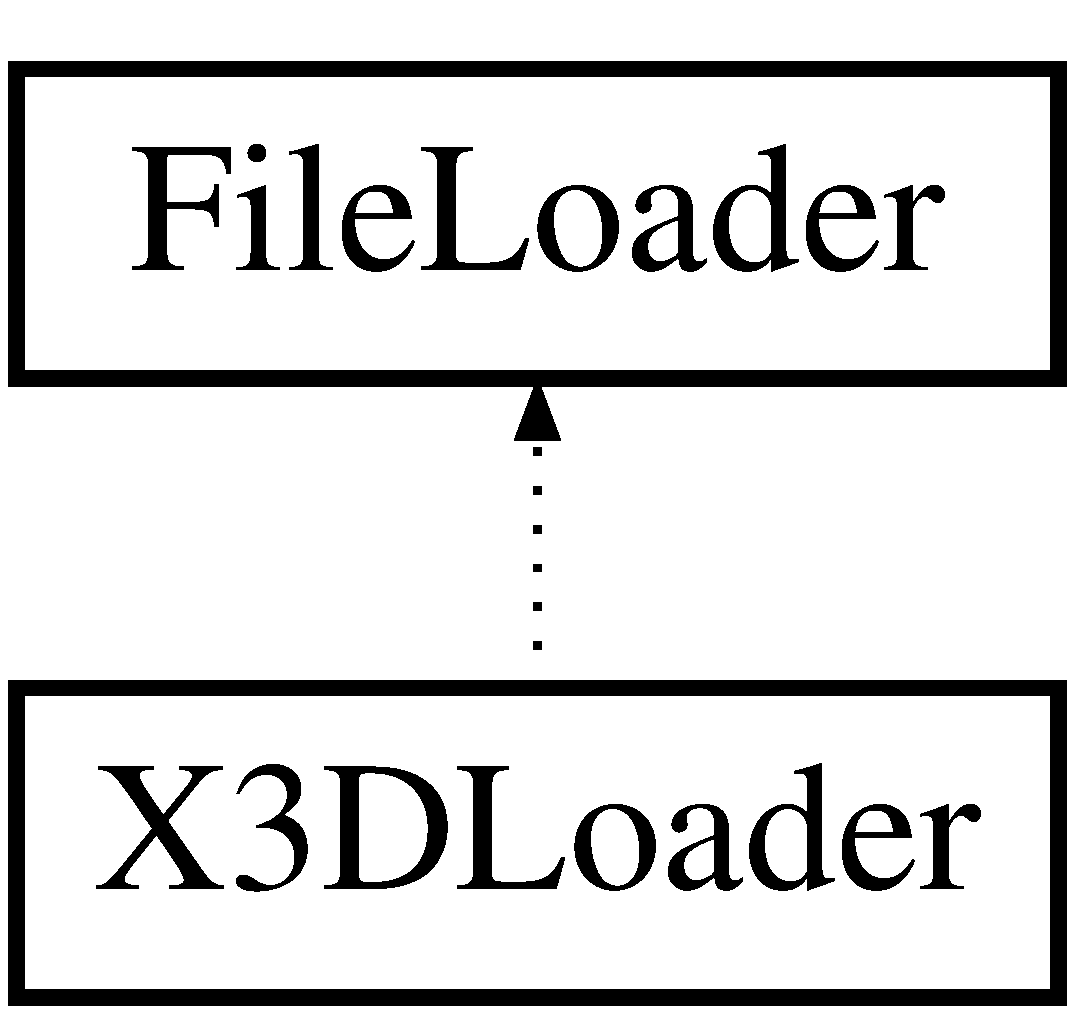
\includegraphics[height=2.000000cm]{classX3DLoader}
\end{center}
\end{figure}
\subsection*{Static Public Member Functions}
\begin{DoxyCompactItemize}
\item 
static \hyperlink{classScene}{Scene} $\ast$ \hyperlink{classX3DLoader_a2693e6c06a6d60e13321e8d9155cc31c}{loadFile} (std::string path)  throw ( std::string )
\end{DoxyCompactItemize}


\subsection{Member Function Documentation}
\hypertarget{classX3DLoader_a2693e6c06a6d60e13321e8d9155cc31c}{
\index{X3DLoader@{X3DLoader}!loadFile@{loadFile}}
\index{loadFile@{loadFile}!X3DLoader@{X3DLoader}}
\subsubsection[{loadFile}]{\setlength{\rightskip}{0pt plus 5cm}{\bf Scene} $\ast$ X3DLoader::loadFile (
\begin{DoxyParamCaption}
\item[{std::string}]{path}
\end{DoxyParamCaption}
)  throw ( std::string )\hspace{0.3cm}{\ttfamily  \mbox{[}static\mbox{]}}}}
\label{classX3DLoader_a2693e6c06a6d60e13321e8d9155cc31c}
Takes a path to an X3D-\/file and returns a scene containing a graphicalobject built from information in the Shape brackets


\begin{DoxyParams}{Parameters}
{\em path} & is the path to the X3D-\/file \\
\hline
\end{DoxyParams}
\begin{DoxyReturn}{Returns}
returns a \hyperlink{classScene}{Scene} object containing the object in the file 
\end{DoxyReturn}


Reimplemented from \hyperlink{classFileLoader_aa10ddbcfa87213ec2d2ade5a51f4cbe0}{FileLoader}.



The documentation for this class was generated from the following files:\begin{DoxyCompactItemize}
\item 
X3DLoader.h\item 
X3DLoader.cpp\end{DoxyCompactItemize}

\printindex
\end{document}
